\baselineskip=8mm
% \renewcommand{\thesubsection}{\thechapter.\arabic{subsection}}
\numberwithin{equation}{chapter}
\numberwithin{equation}{section}
\renewcommand{\thesubsection}{\arabic{subsection}.}
\renewcommand{\theequation}{\thesection.\arabic{equation}}
\renewcommand{\thesection}{}
\renewcommand{\thesubsubsection}{\thesubsection\arabic{subsubsection}.}




\section{การออกแบบส่วนเชื่อมต่อประสานกับผู้ใช้}

ในการออกแบบส่วนต่อประสานกับผู้ใช้ของแอปพลิเคชันจัดตารางเวรพยาบาลจะเน้นไปที่ความเรียบง่าย สบายตา และใช้งานได้ง่าย เพื่อให้บุคคลากรณ์ทางการแพทย์ใช้ได้ง่ายและรวดเร็ว โดยจะมีการออกแบบหน้าจอต่างๆได้ดังนี้

\vspace{1.5cm}


\begin{figure}[h]
    \centering
    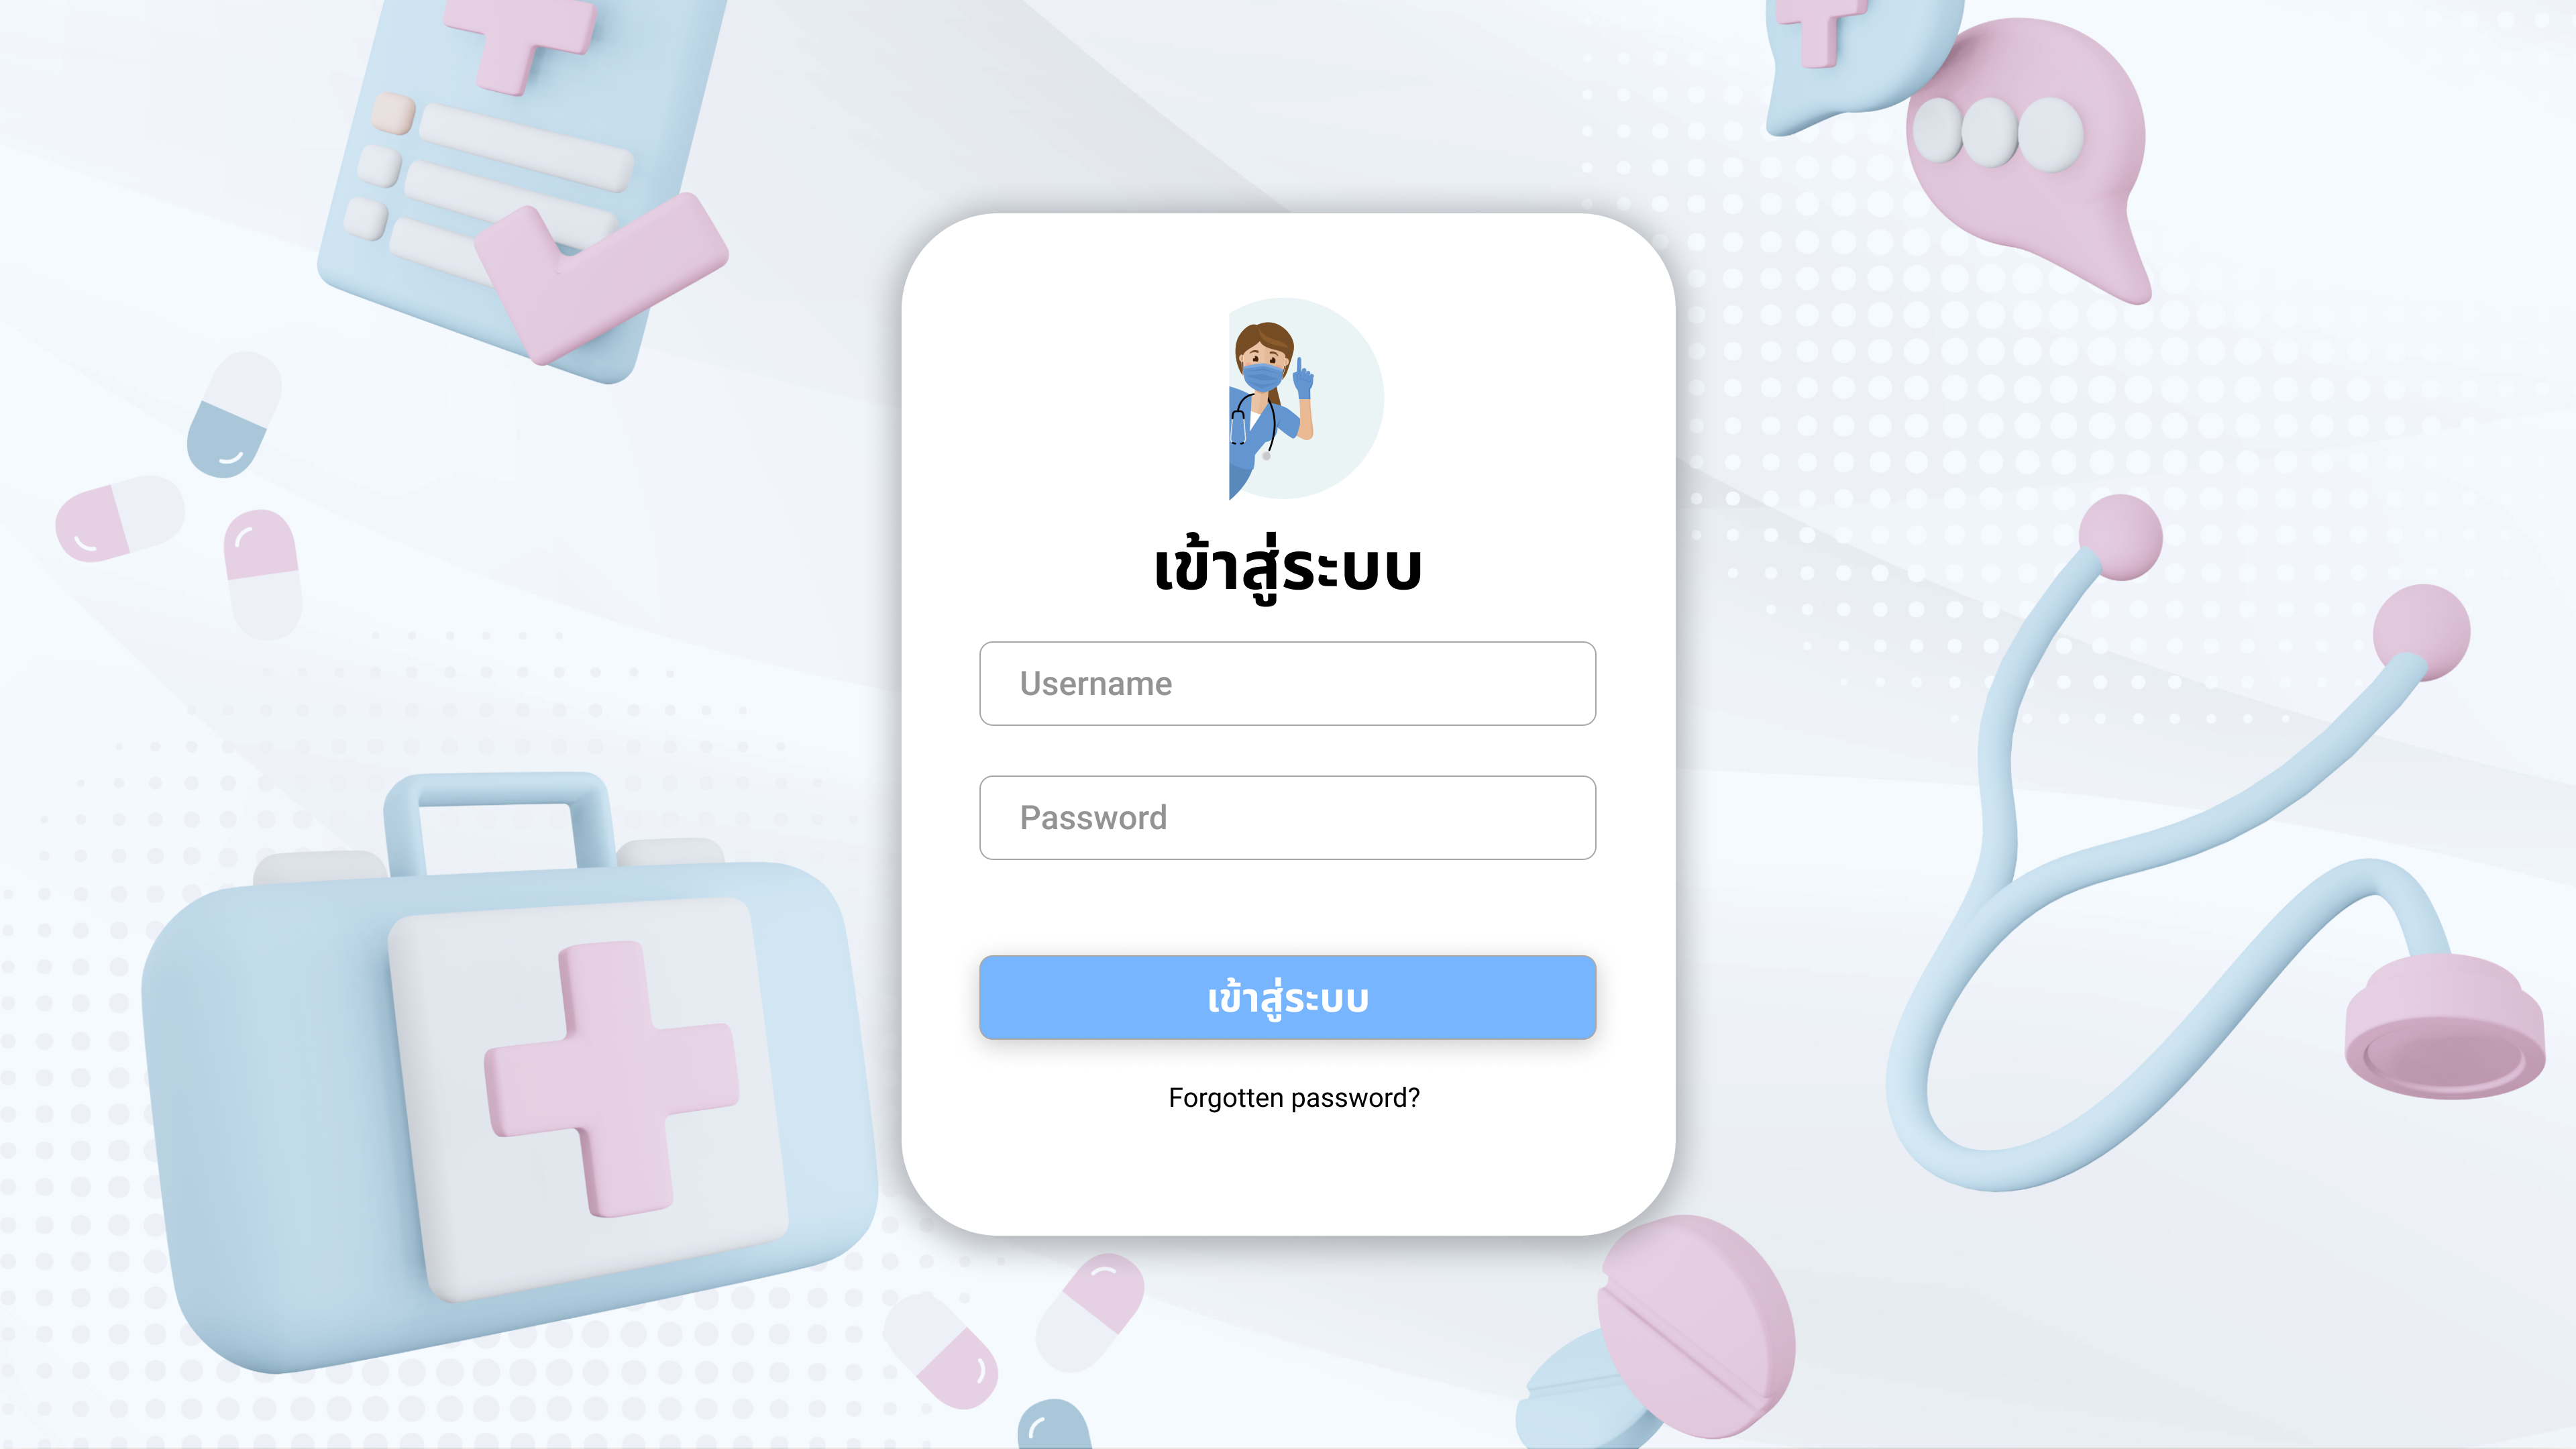
\includegraphics[width=0.7\textwidth]{Login ui.png}
    \caption{แสดงหน้าการเข้าสู่ระบบ}
    \end{figure}

\begin{figure}
    \centering
    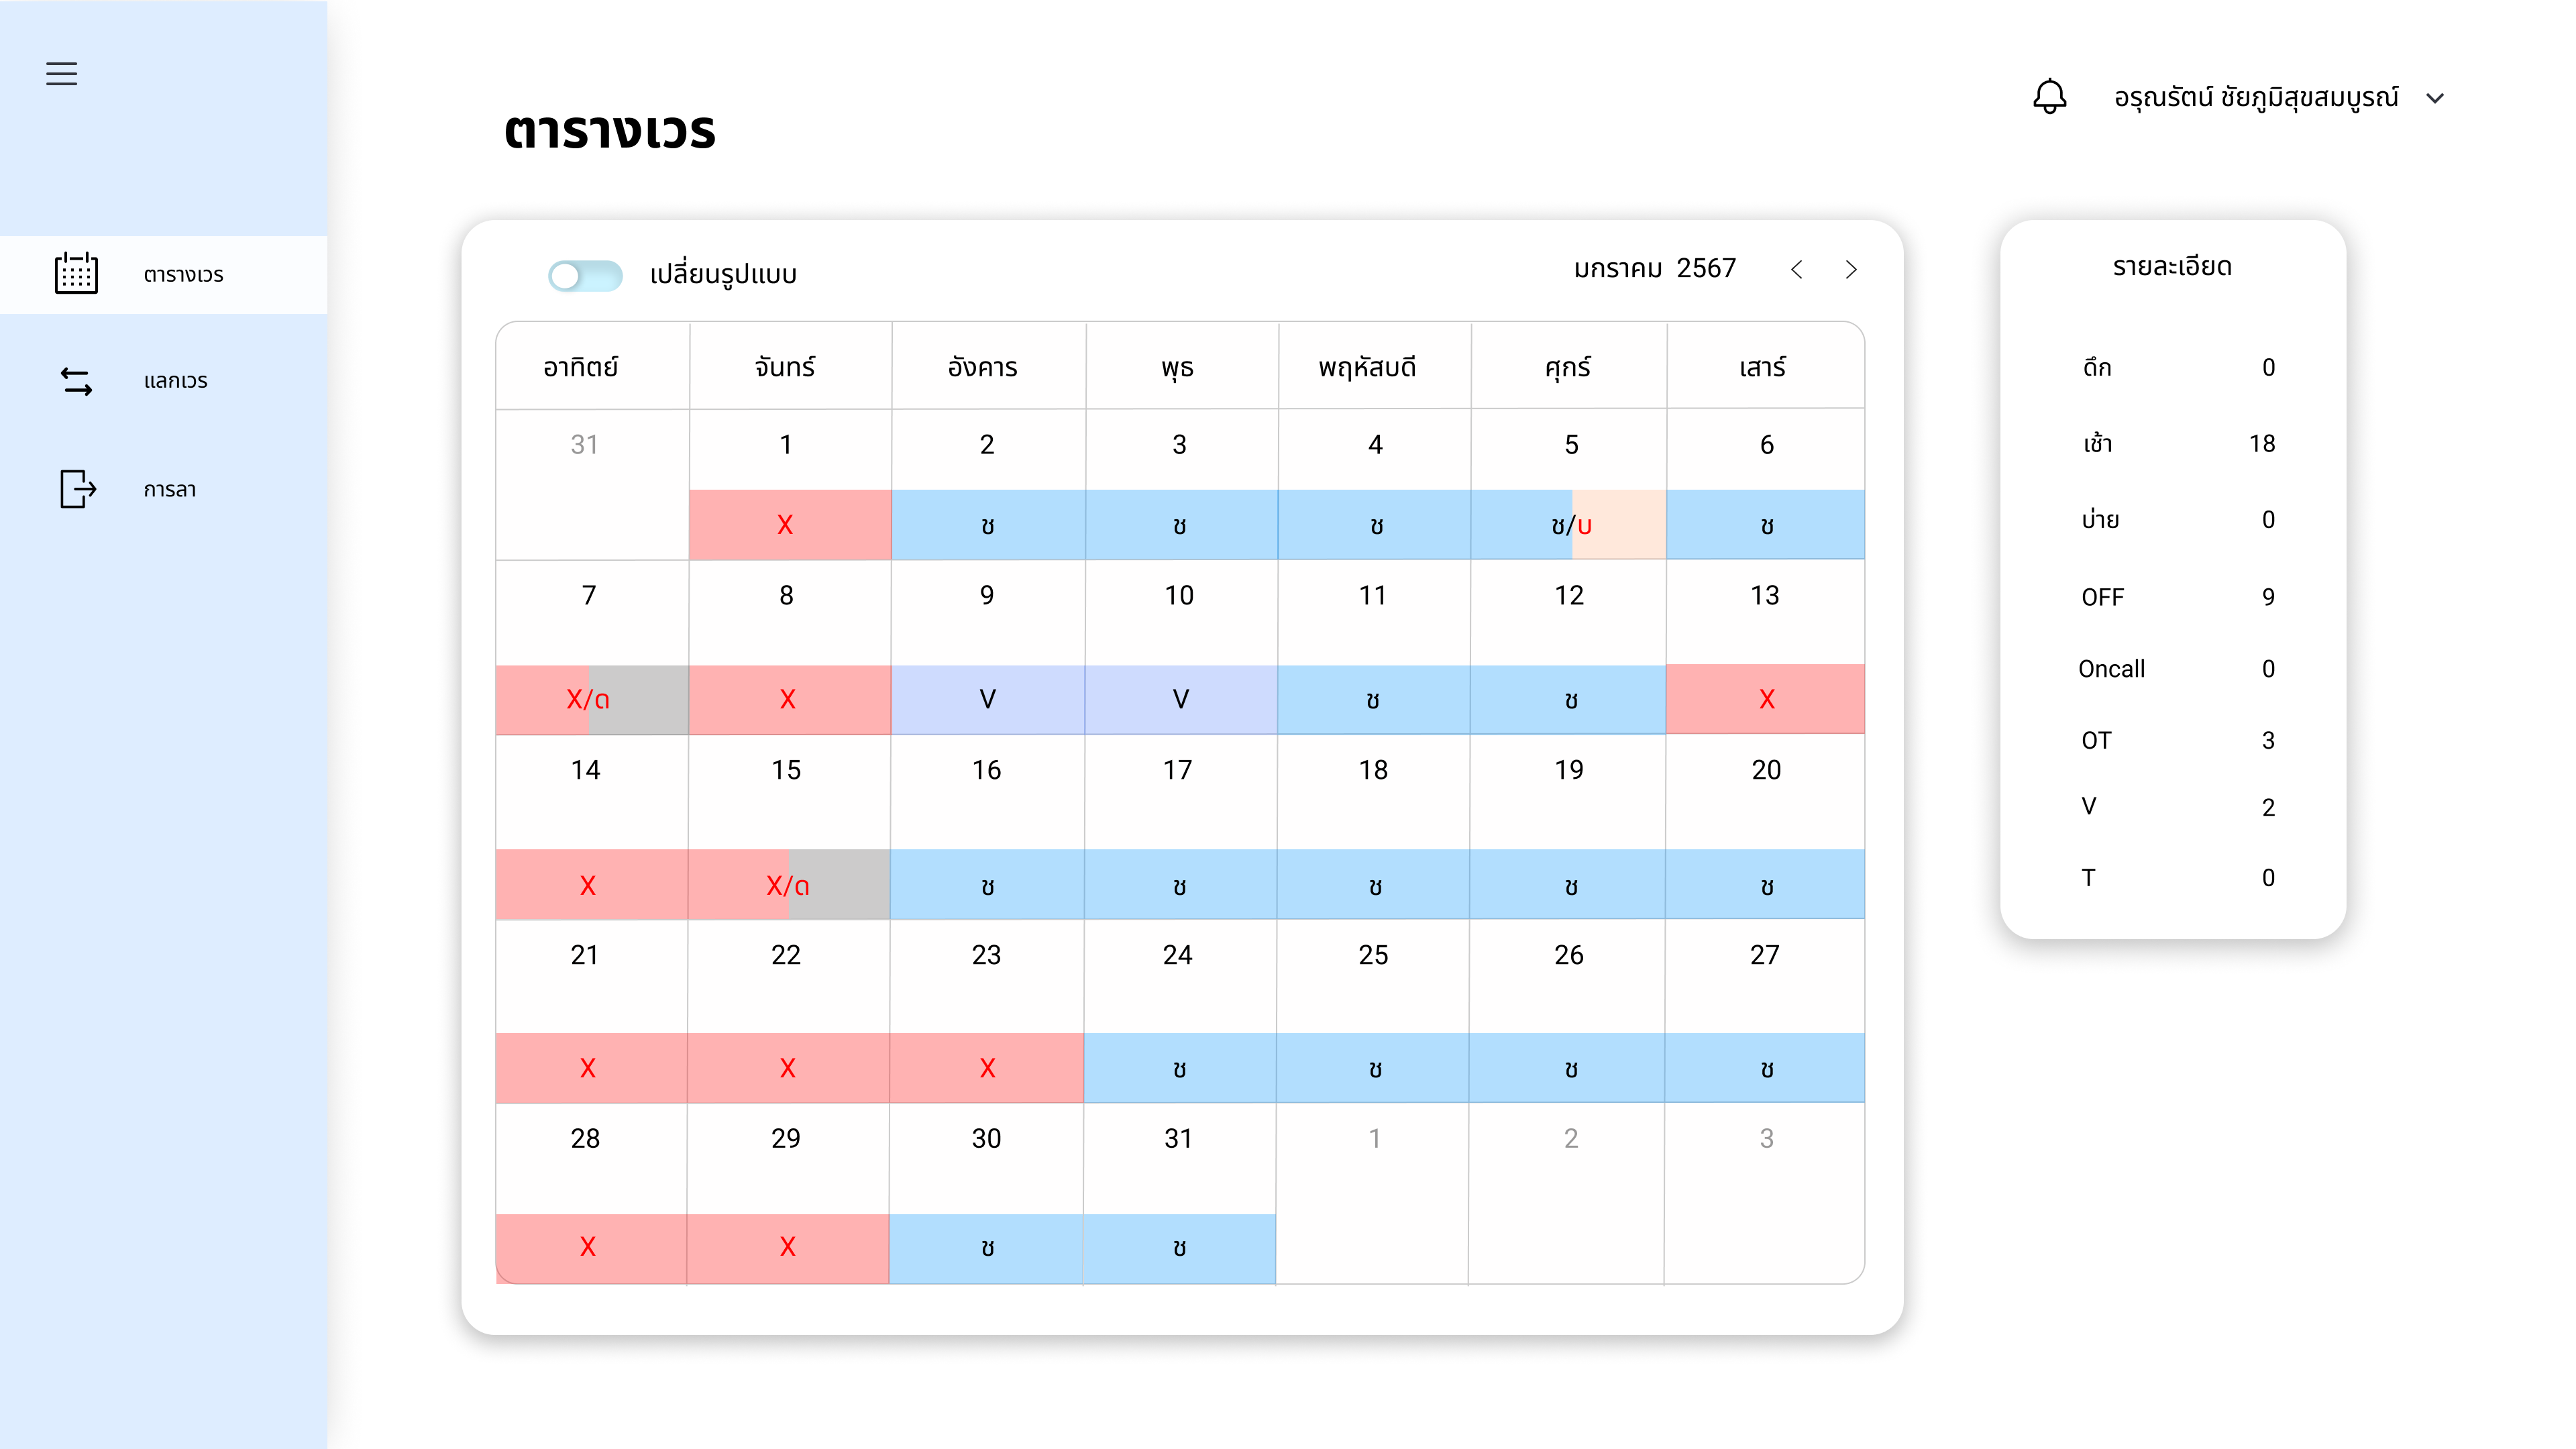
\includegraphics[width=0.7\textwidth]{Home ui.png}
    \caption{แสดงหน้าตารางเวร}
\end{figure}

\begin{figure}
    \centering
    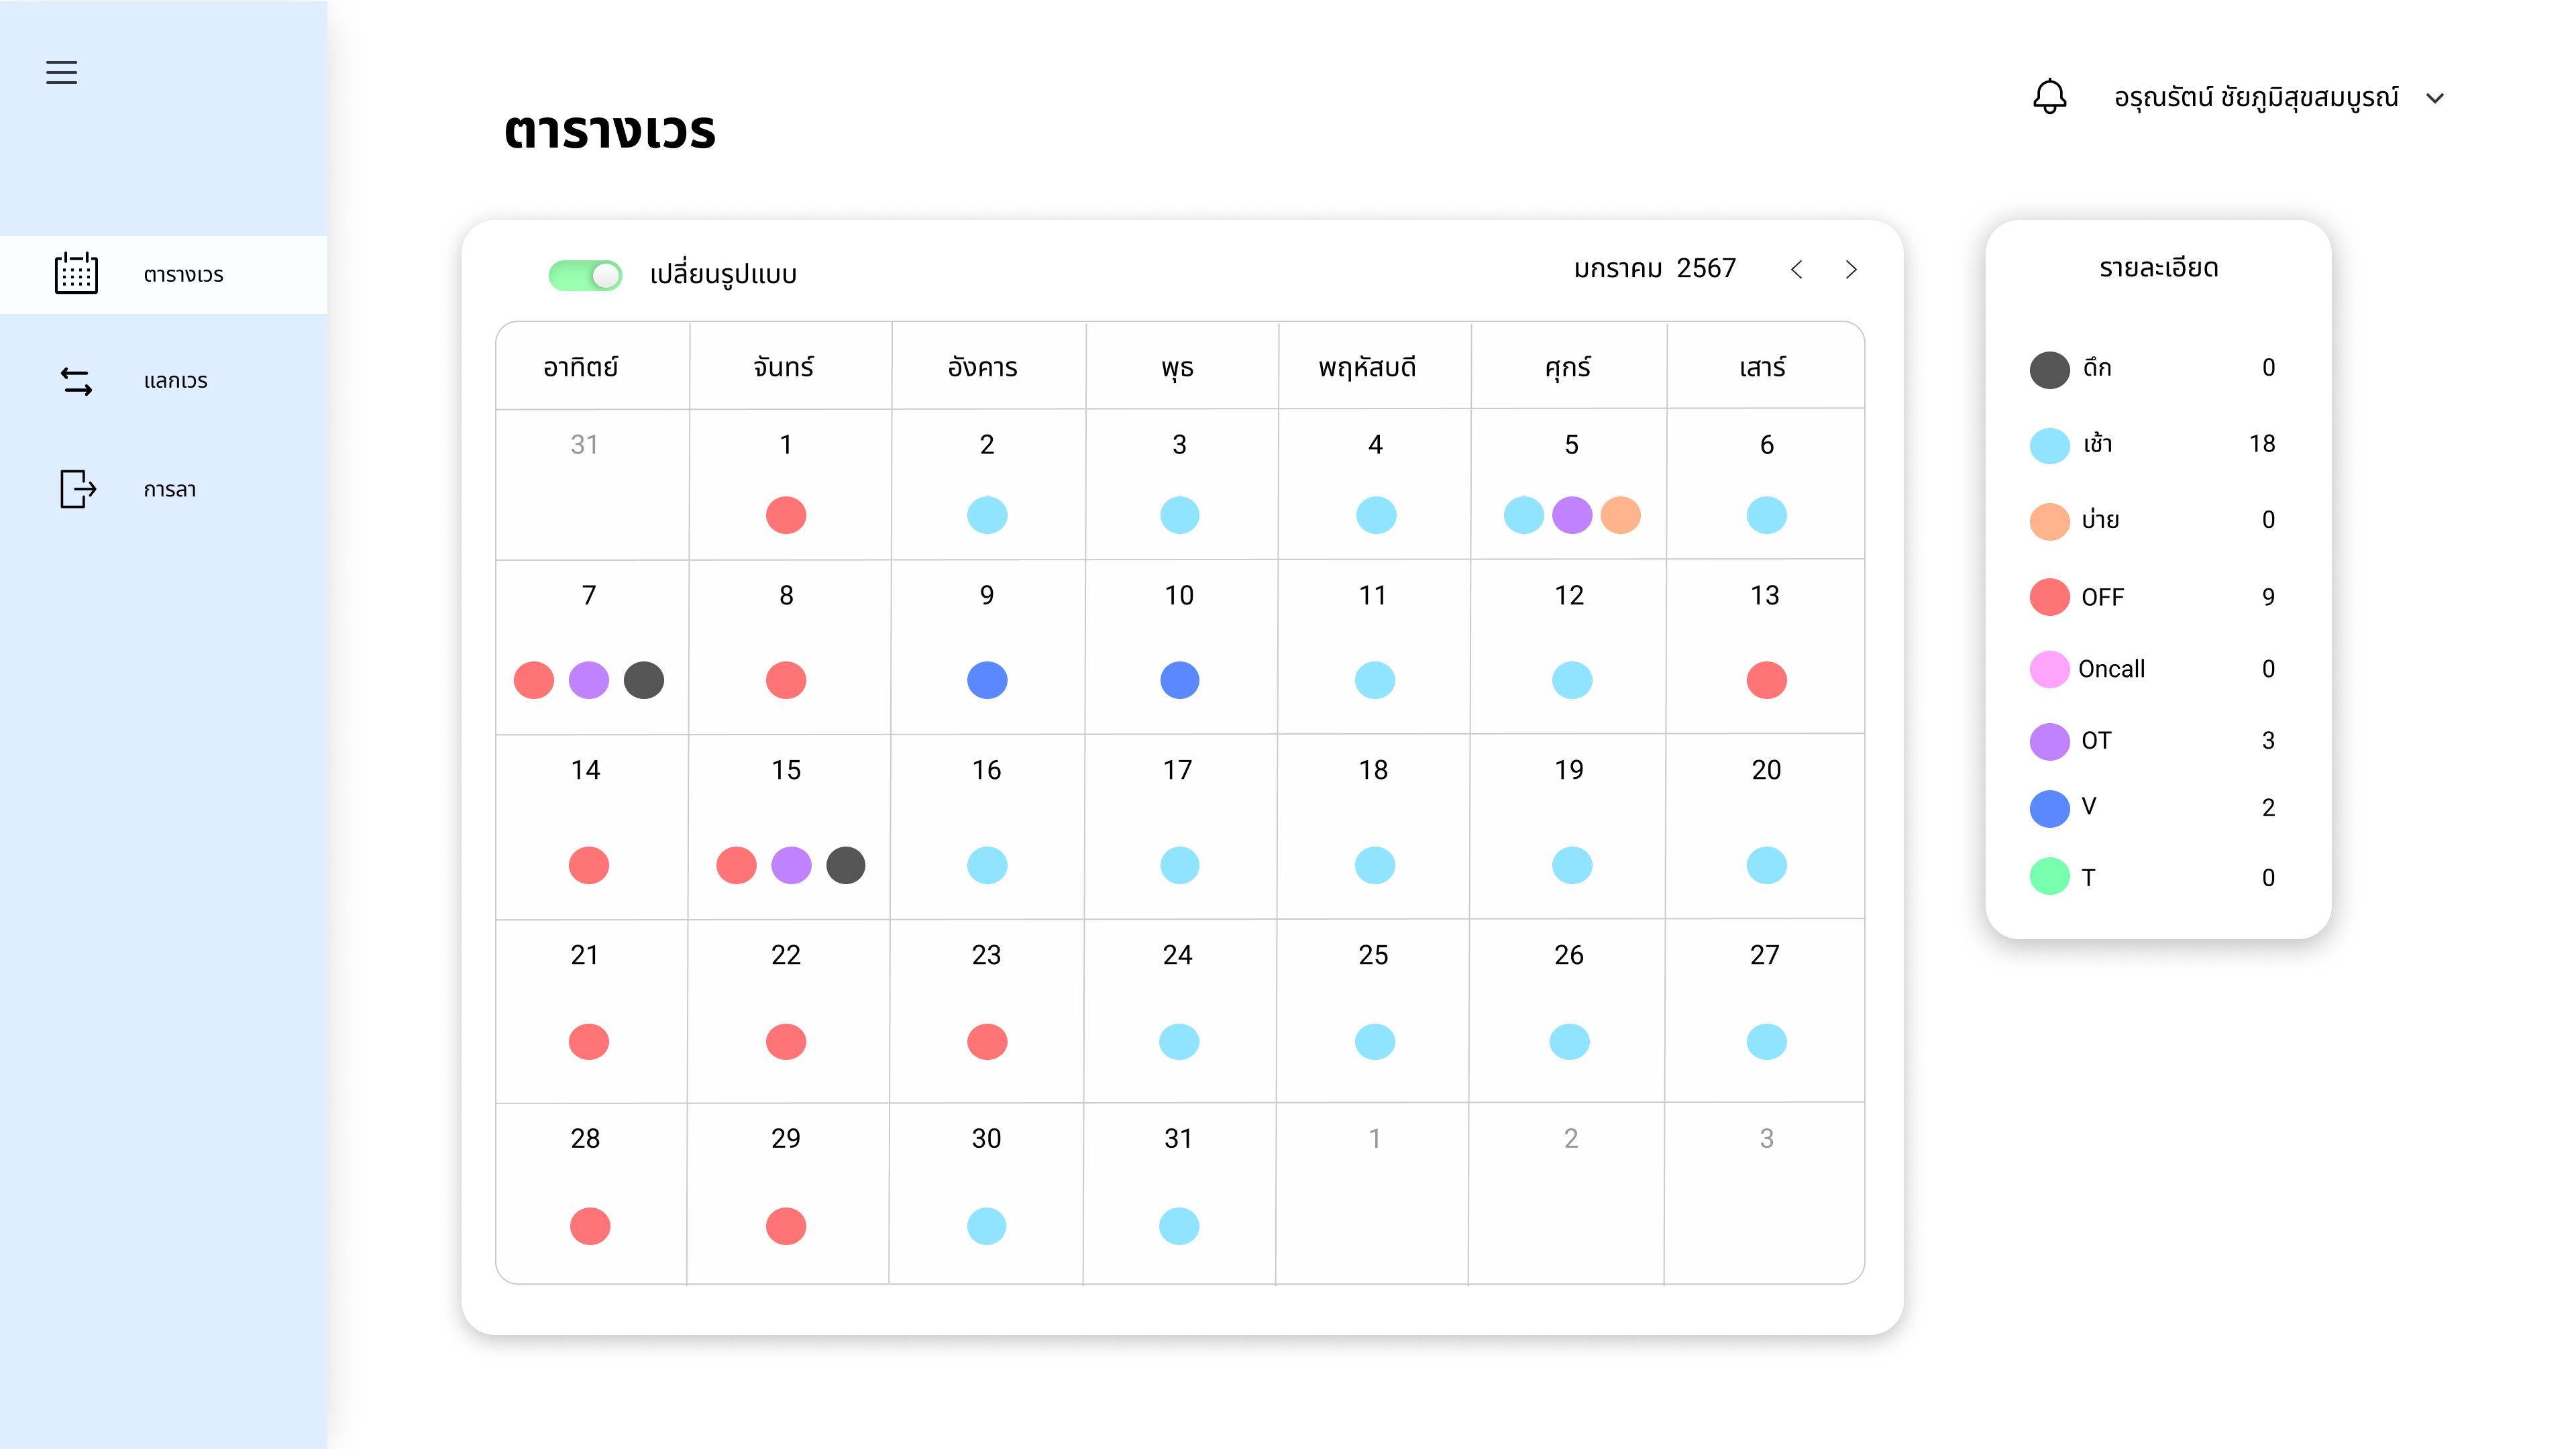
\includegraphics[width=0.8\textwidth]{3 ui.png}
    \caption{แสดงหน้าตารางเวร}
\end{figure}

\begin{figure}
    \centering
    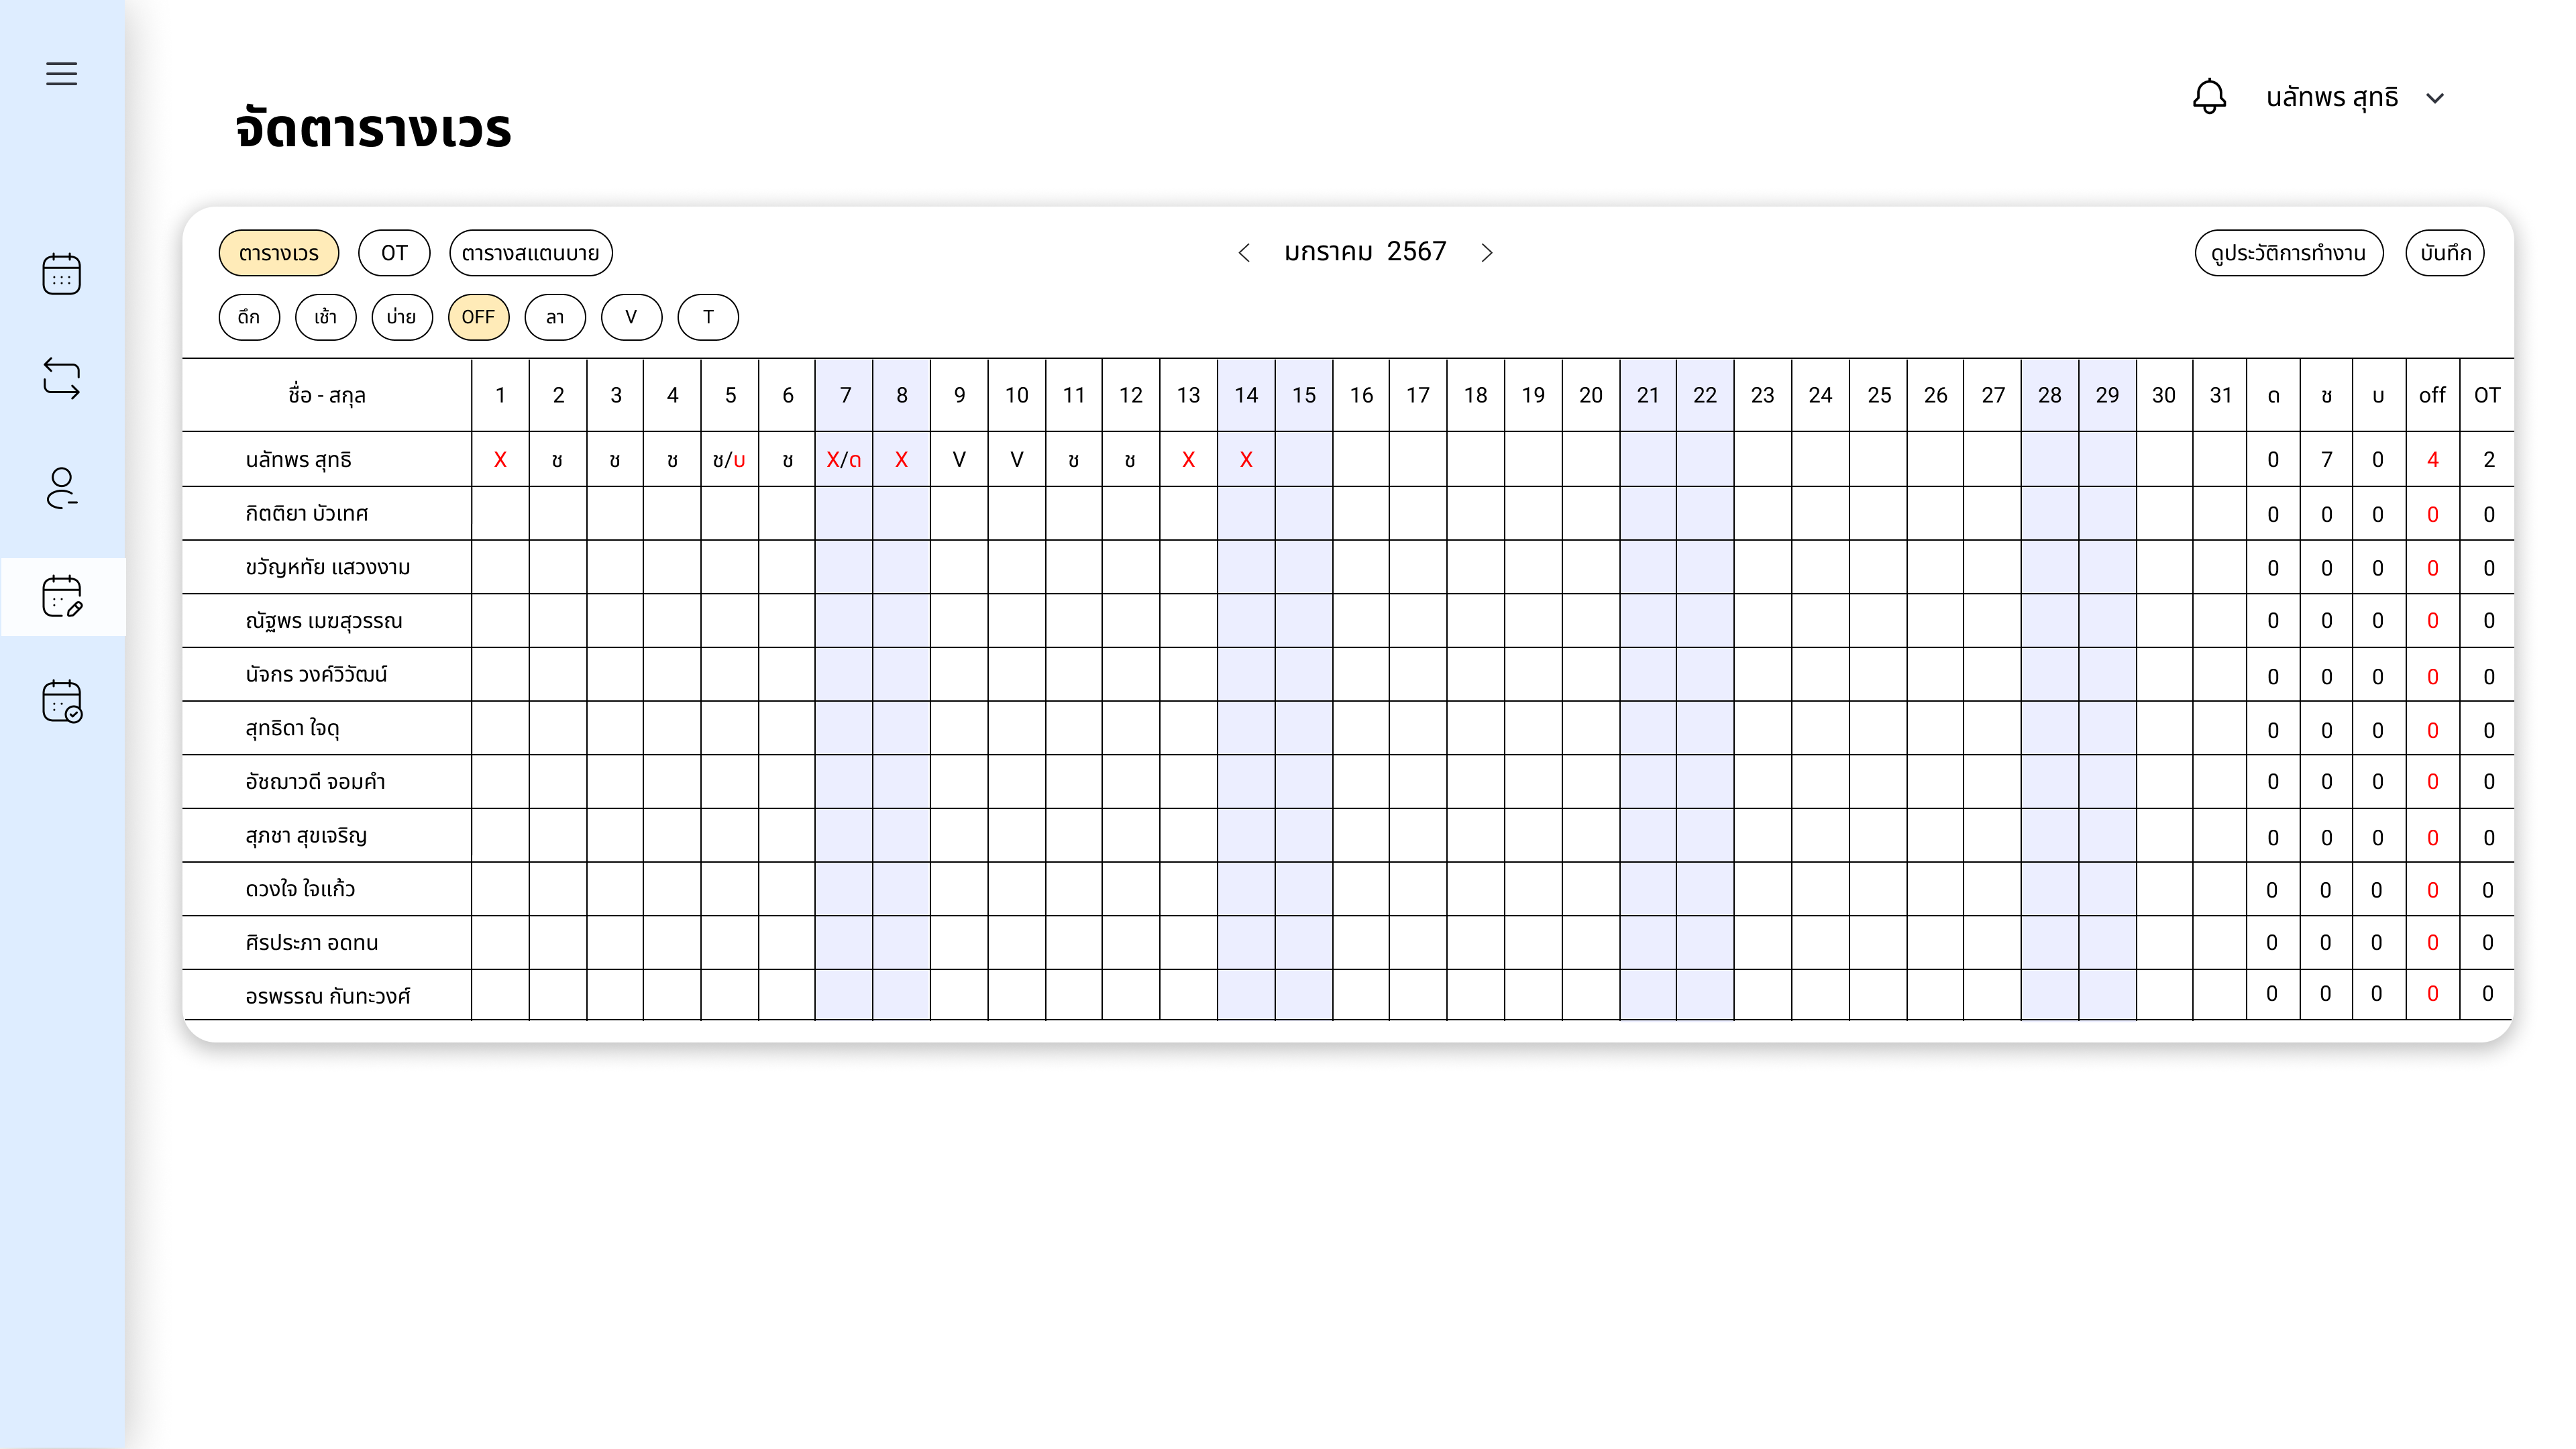
\includegraphics[width=0.8\textwidth]{4ui.png}
    \caption{แสดงหน้าจัดตารางเวร}
\end{figure}

\begin{figure}
    \centering
    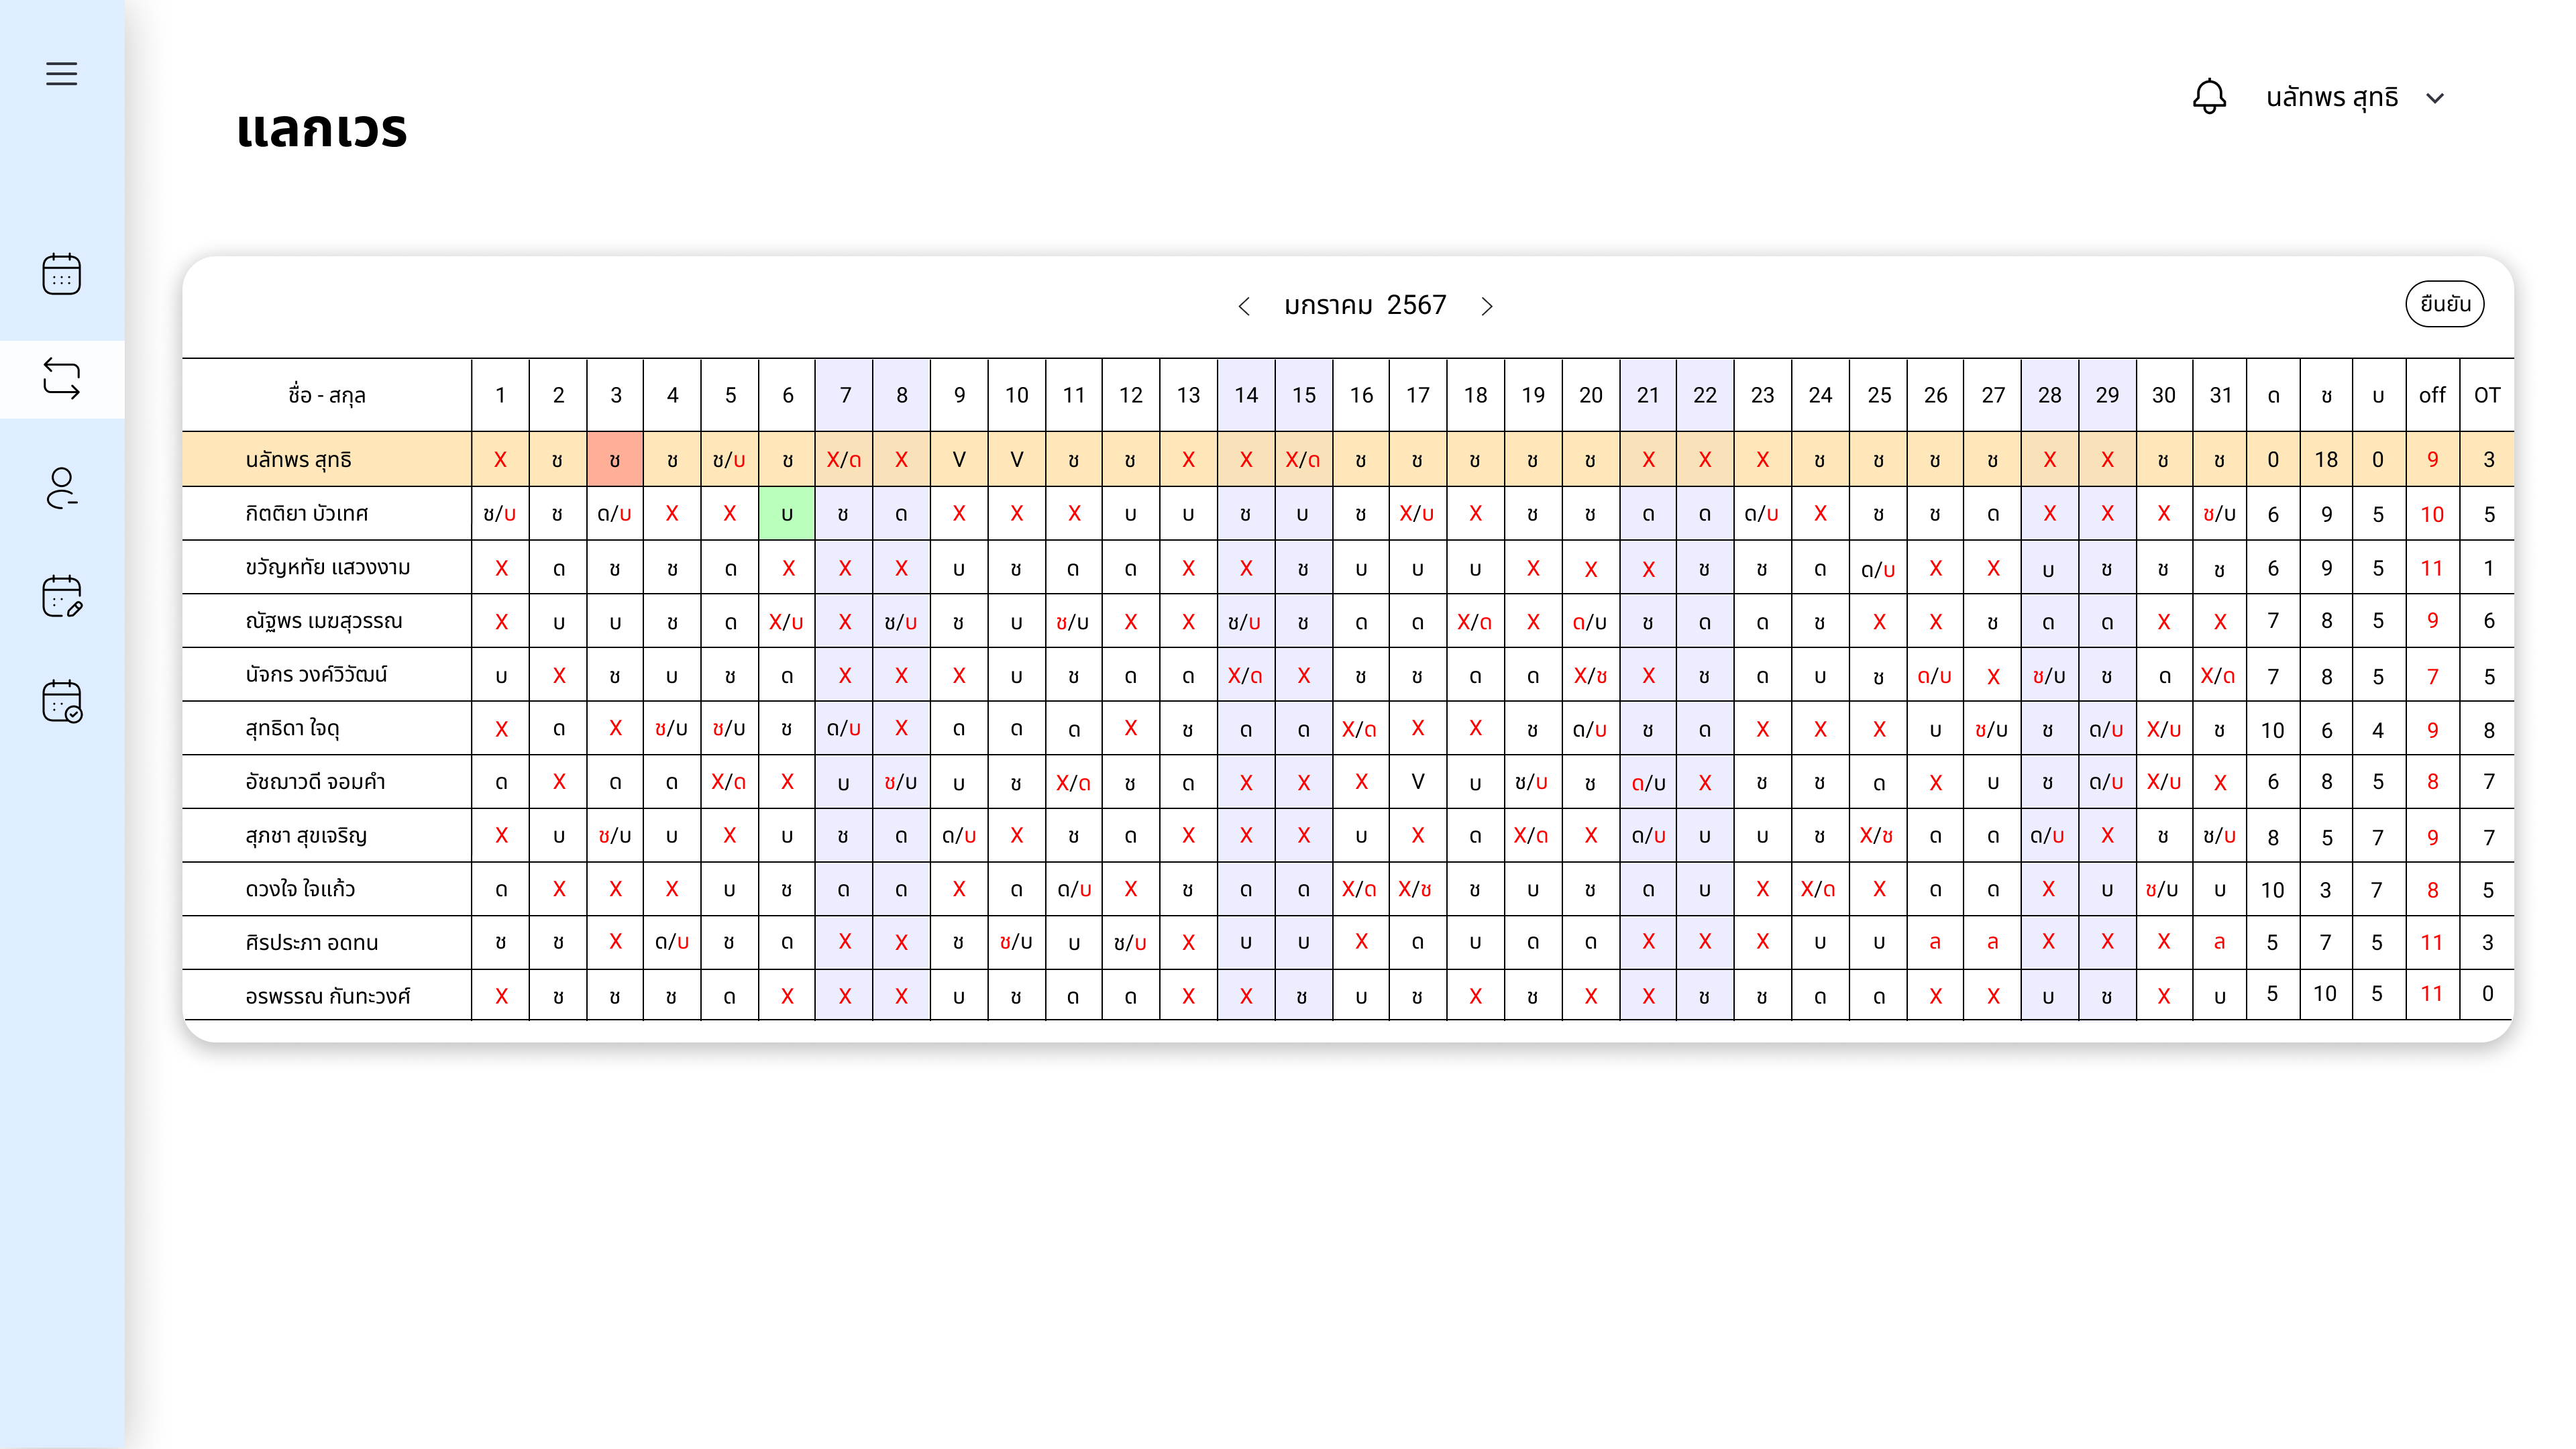
\includegraphics[width=0.8\textwidth]{5ui.png}
    \caption{แสดงหน้าการแลกเวร}
\end{figure}

\begin{figure}
    \centering
    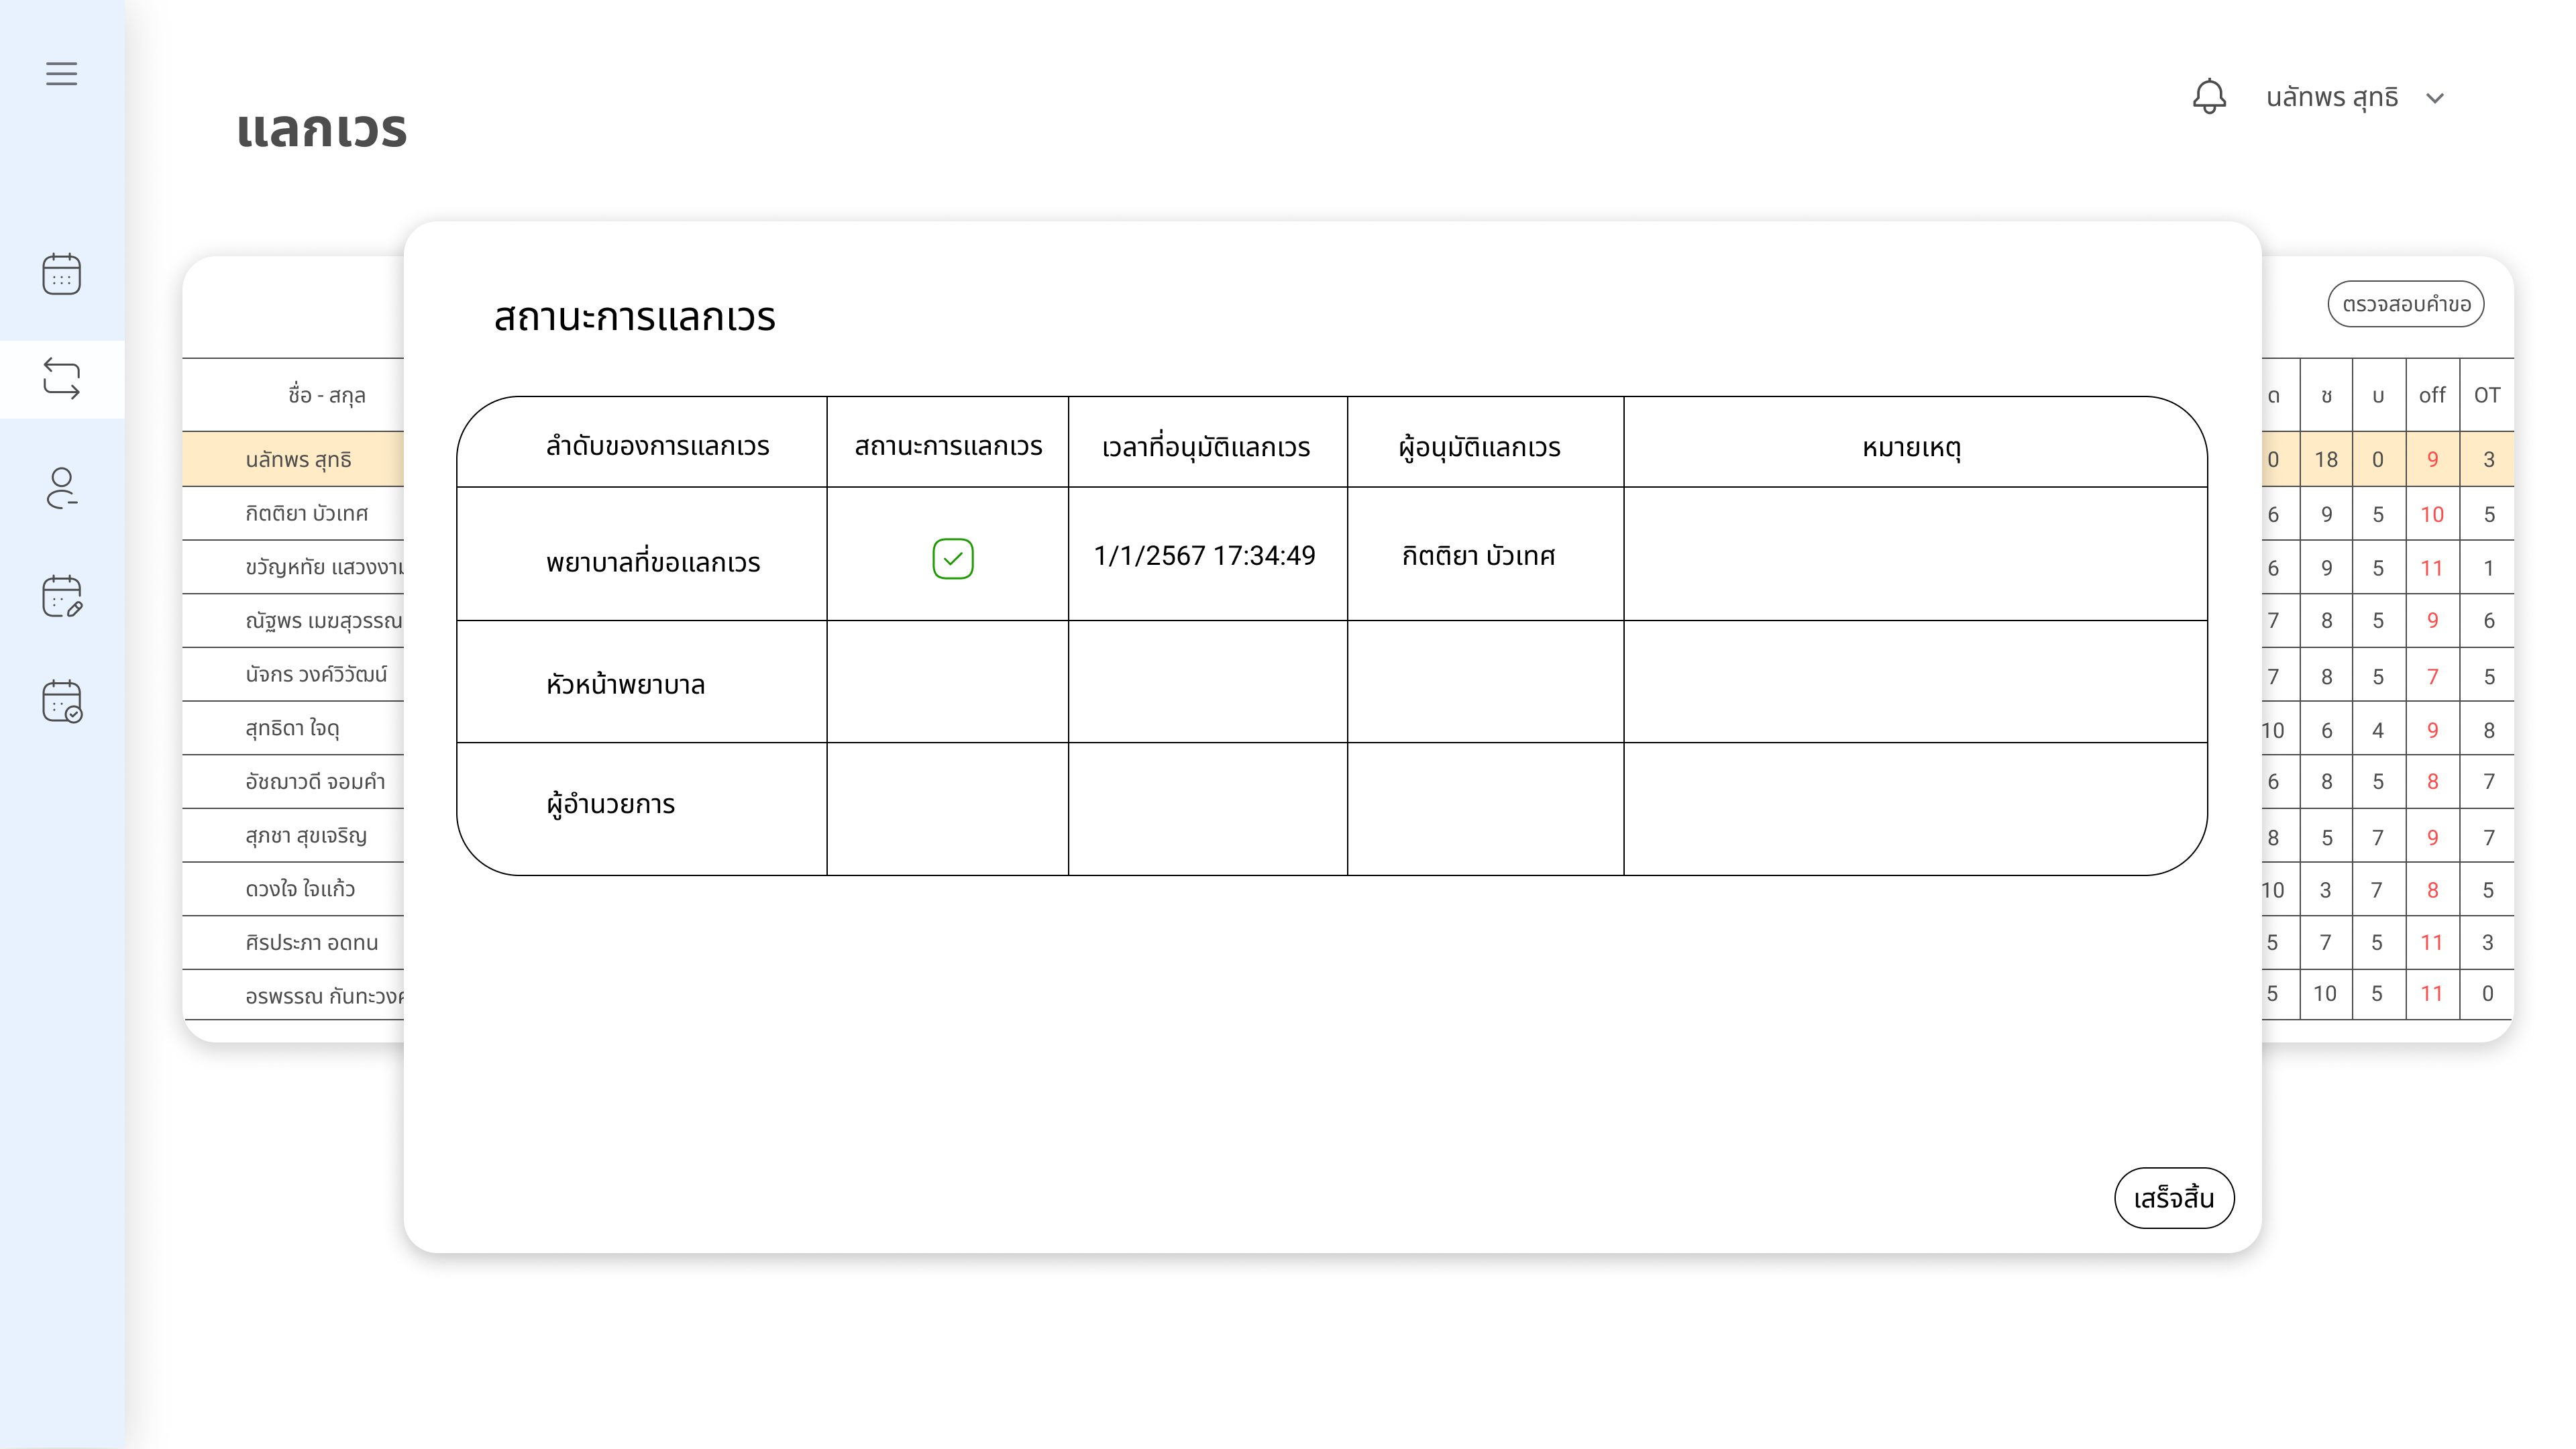
\includegraphics[width=0.8\textwidth]{6ui.png}
    \caption{แสดงหน้าสถานะการแลกเวร}
\end{figure}

\begin{figure}
    \centering
    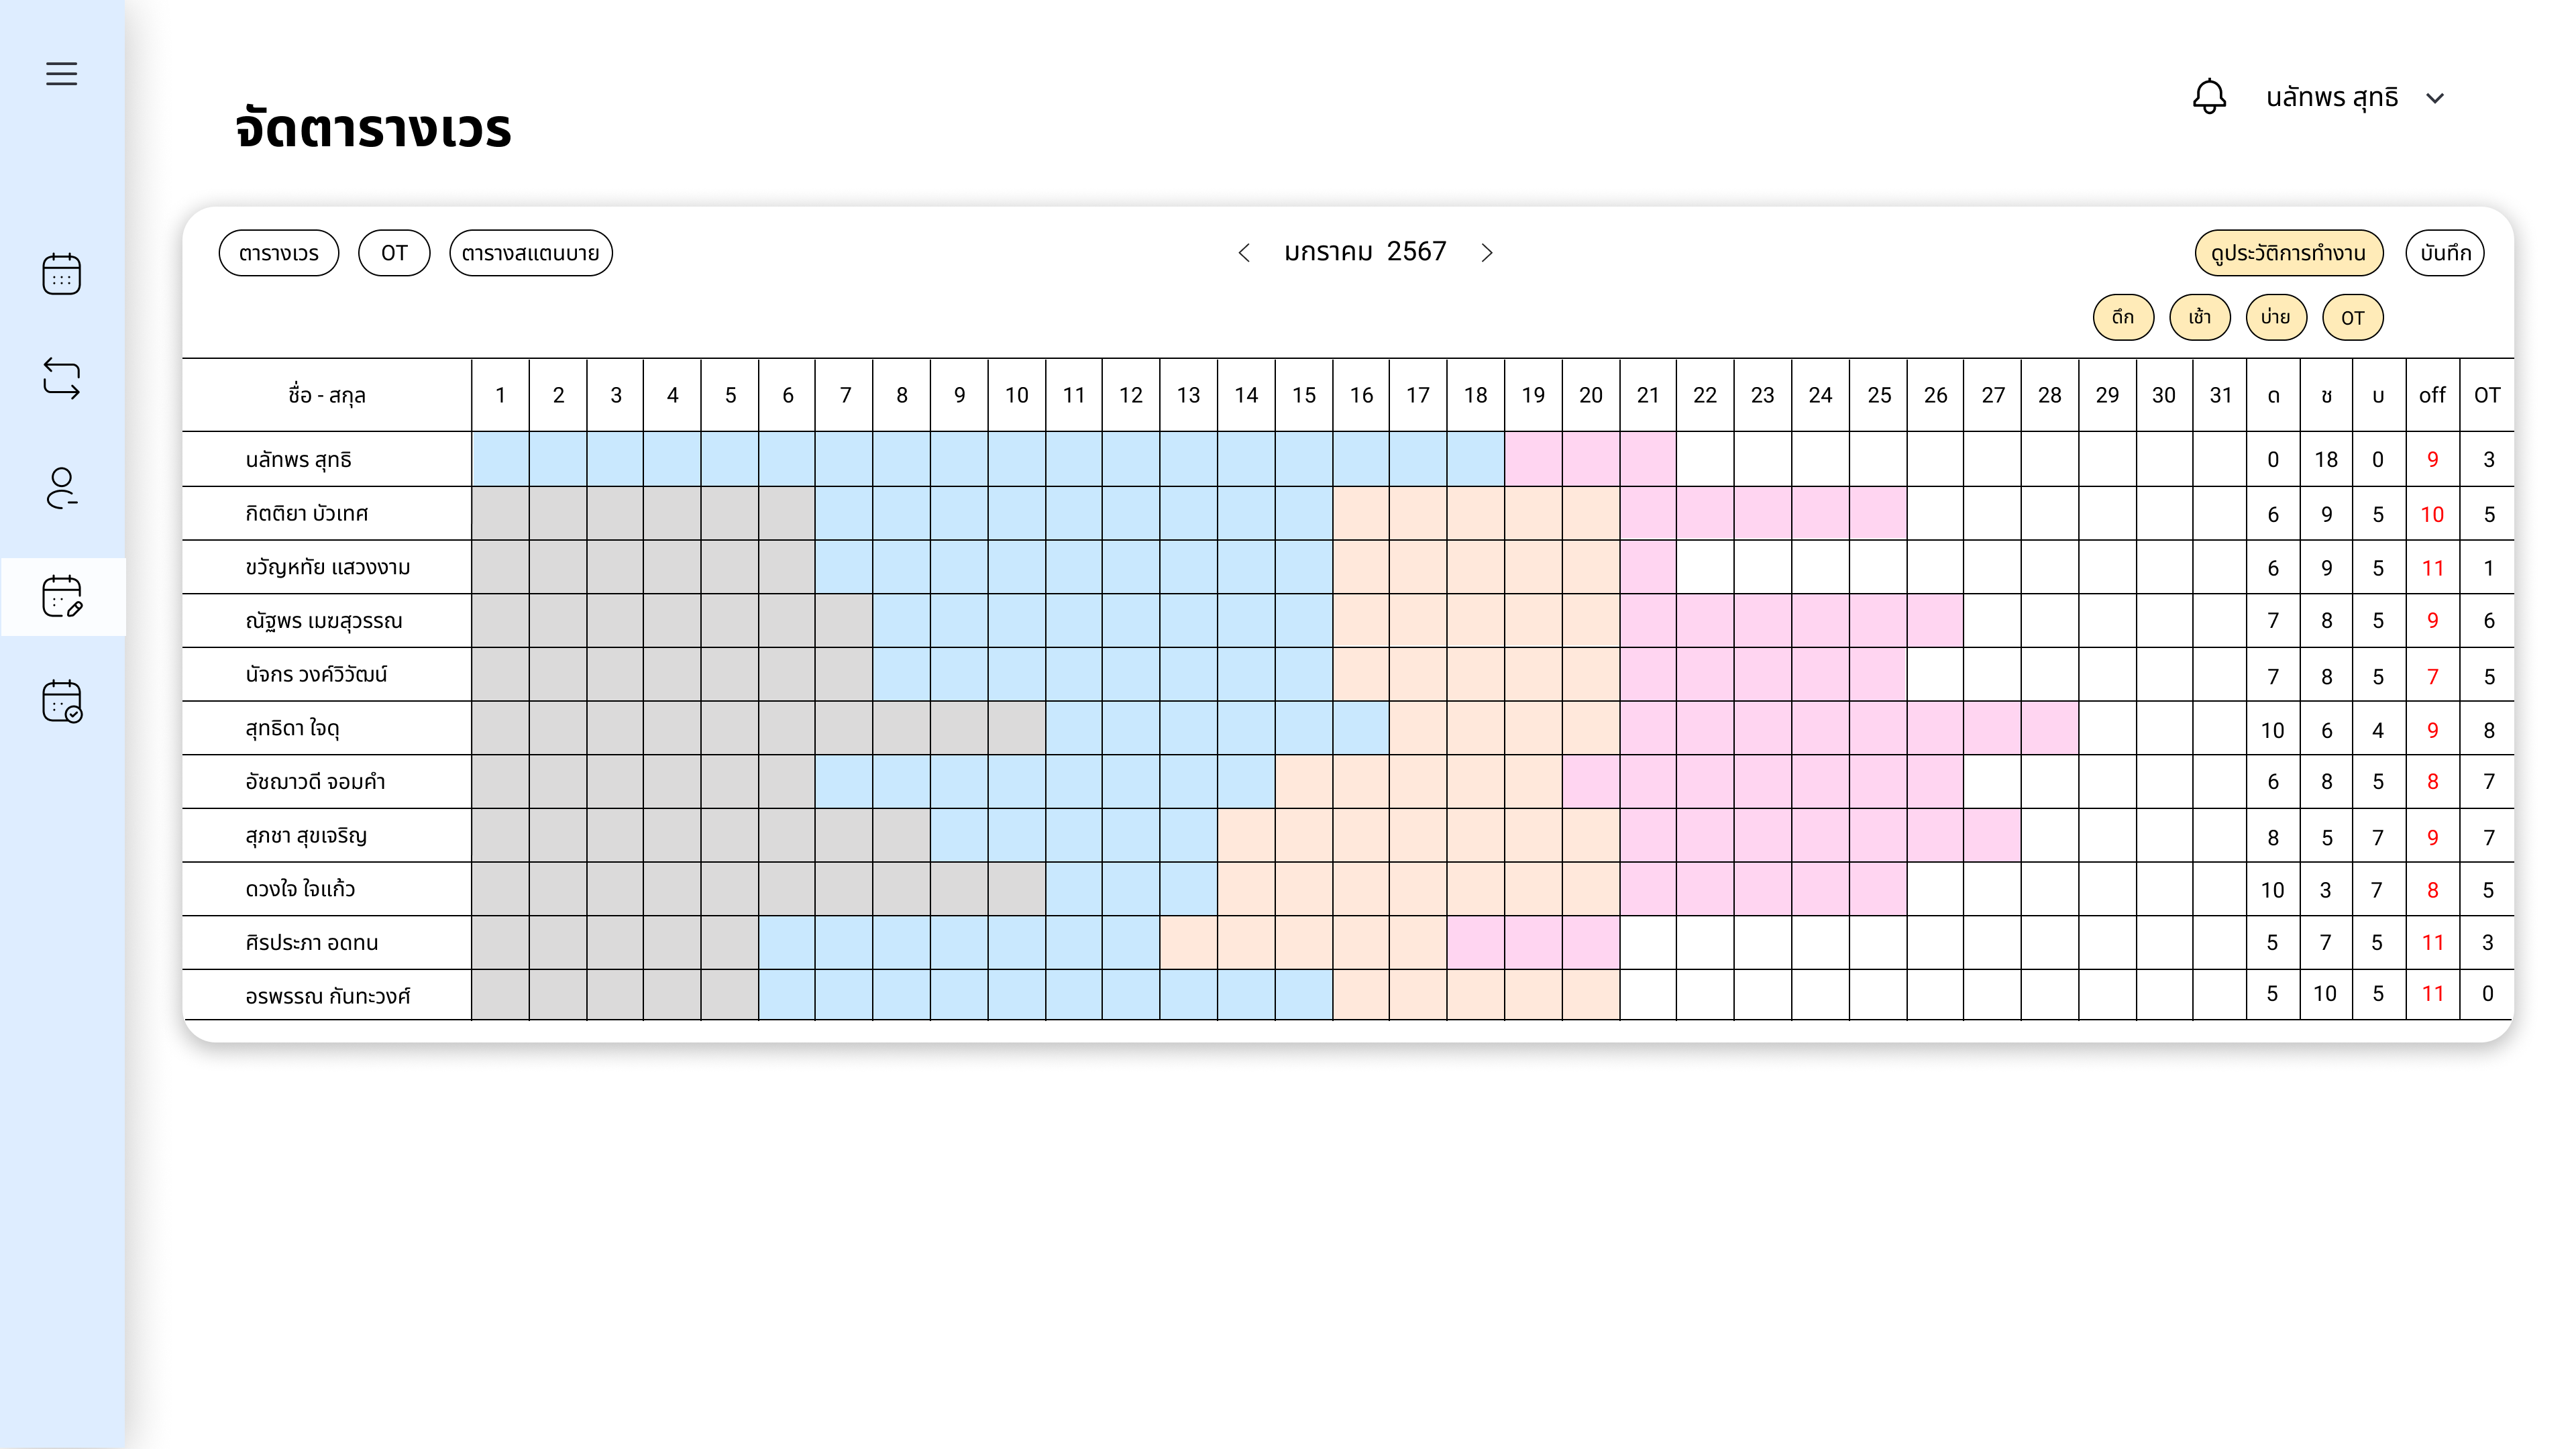
\includegraphics[width=0.8\textwidth]{7ui.png}
    \caption{แสดงหน้าประวัติการทำงานของพยาบาล}
\end{figure}

\begin{figure}
    \centering
    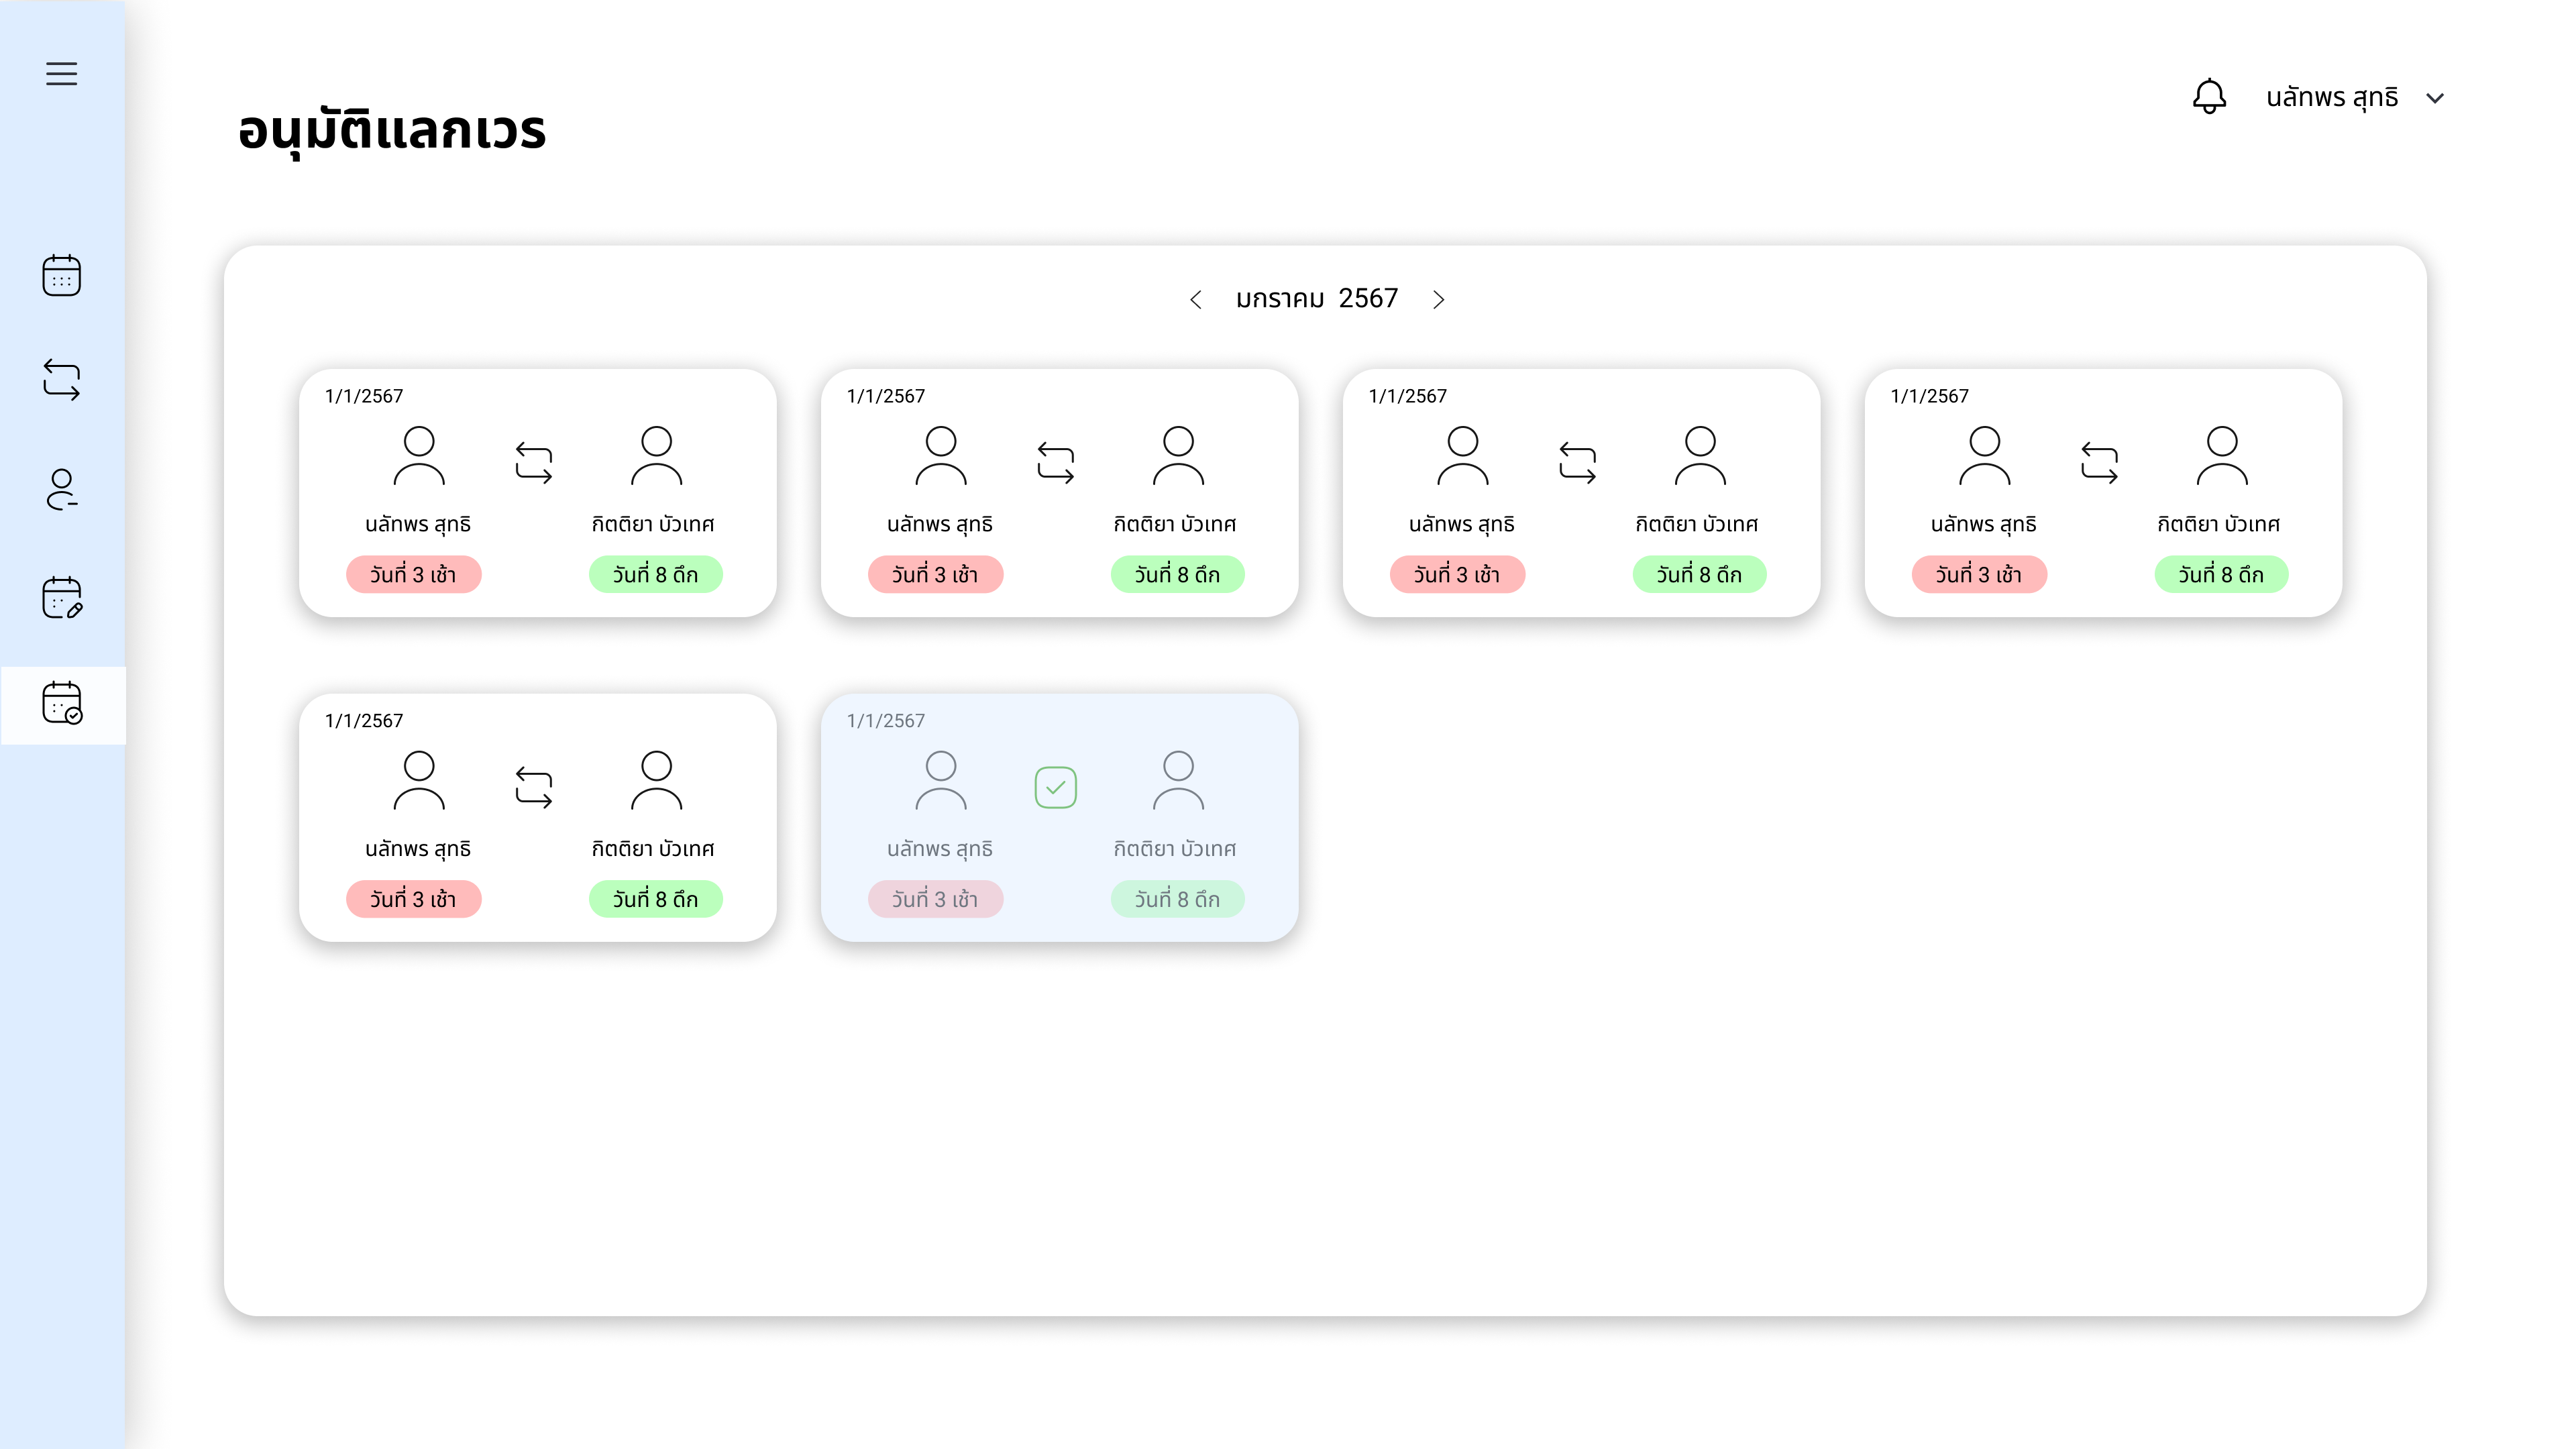
\includegraphics[width=0.8\textwidth]{8ui.png}
    \caption{แสดงหน้าอนุมัติการแลกเวร}
\end{figure}

\begin{figure}
    \centering
    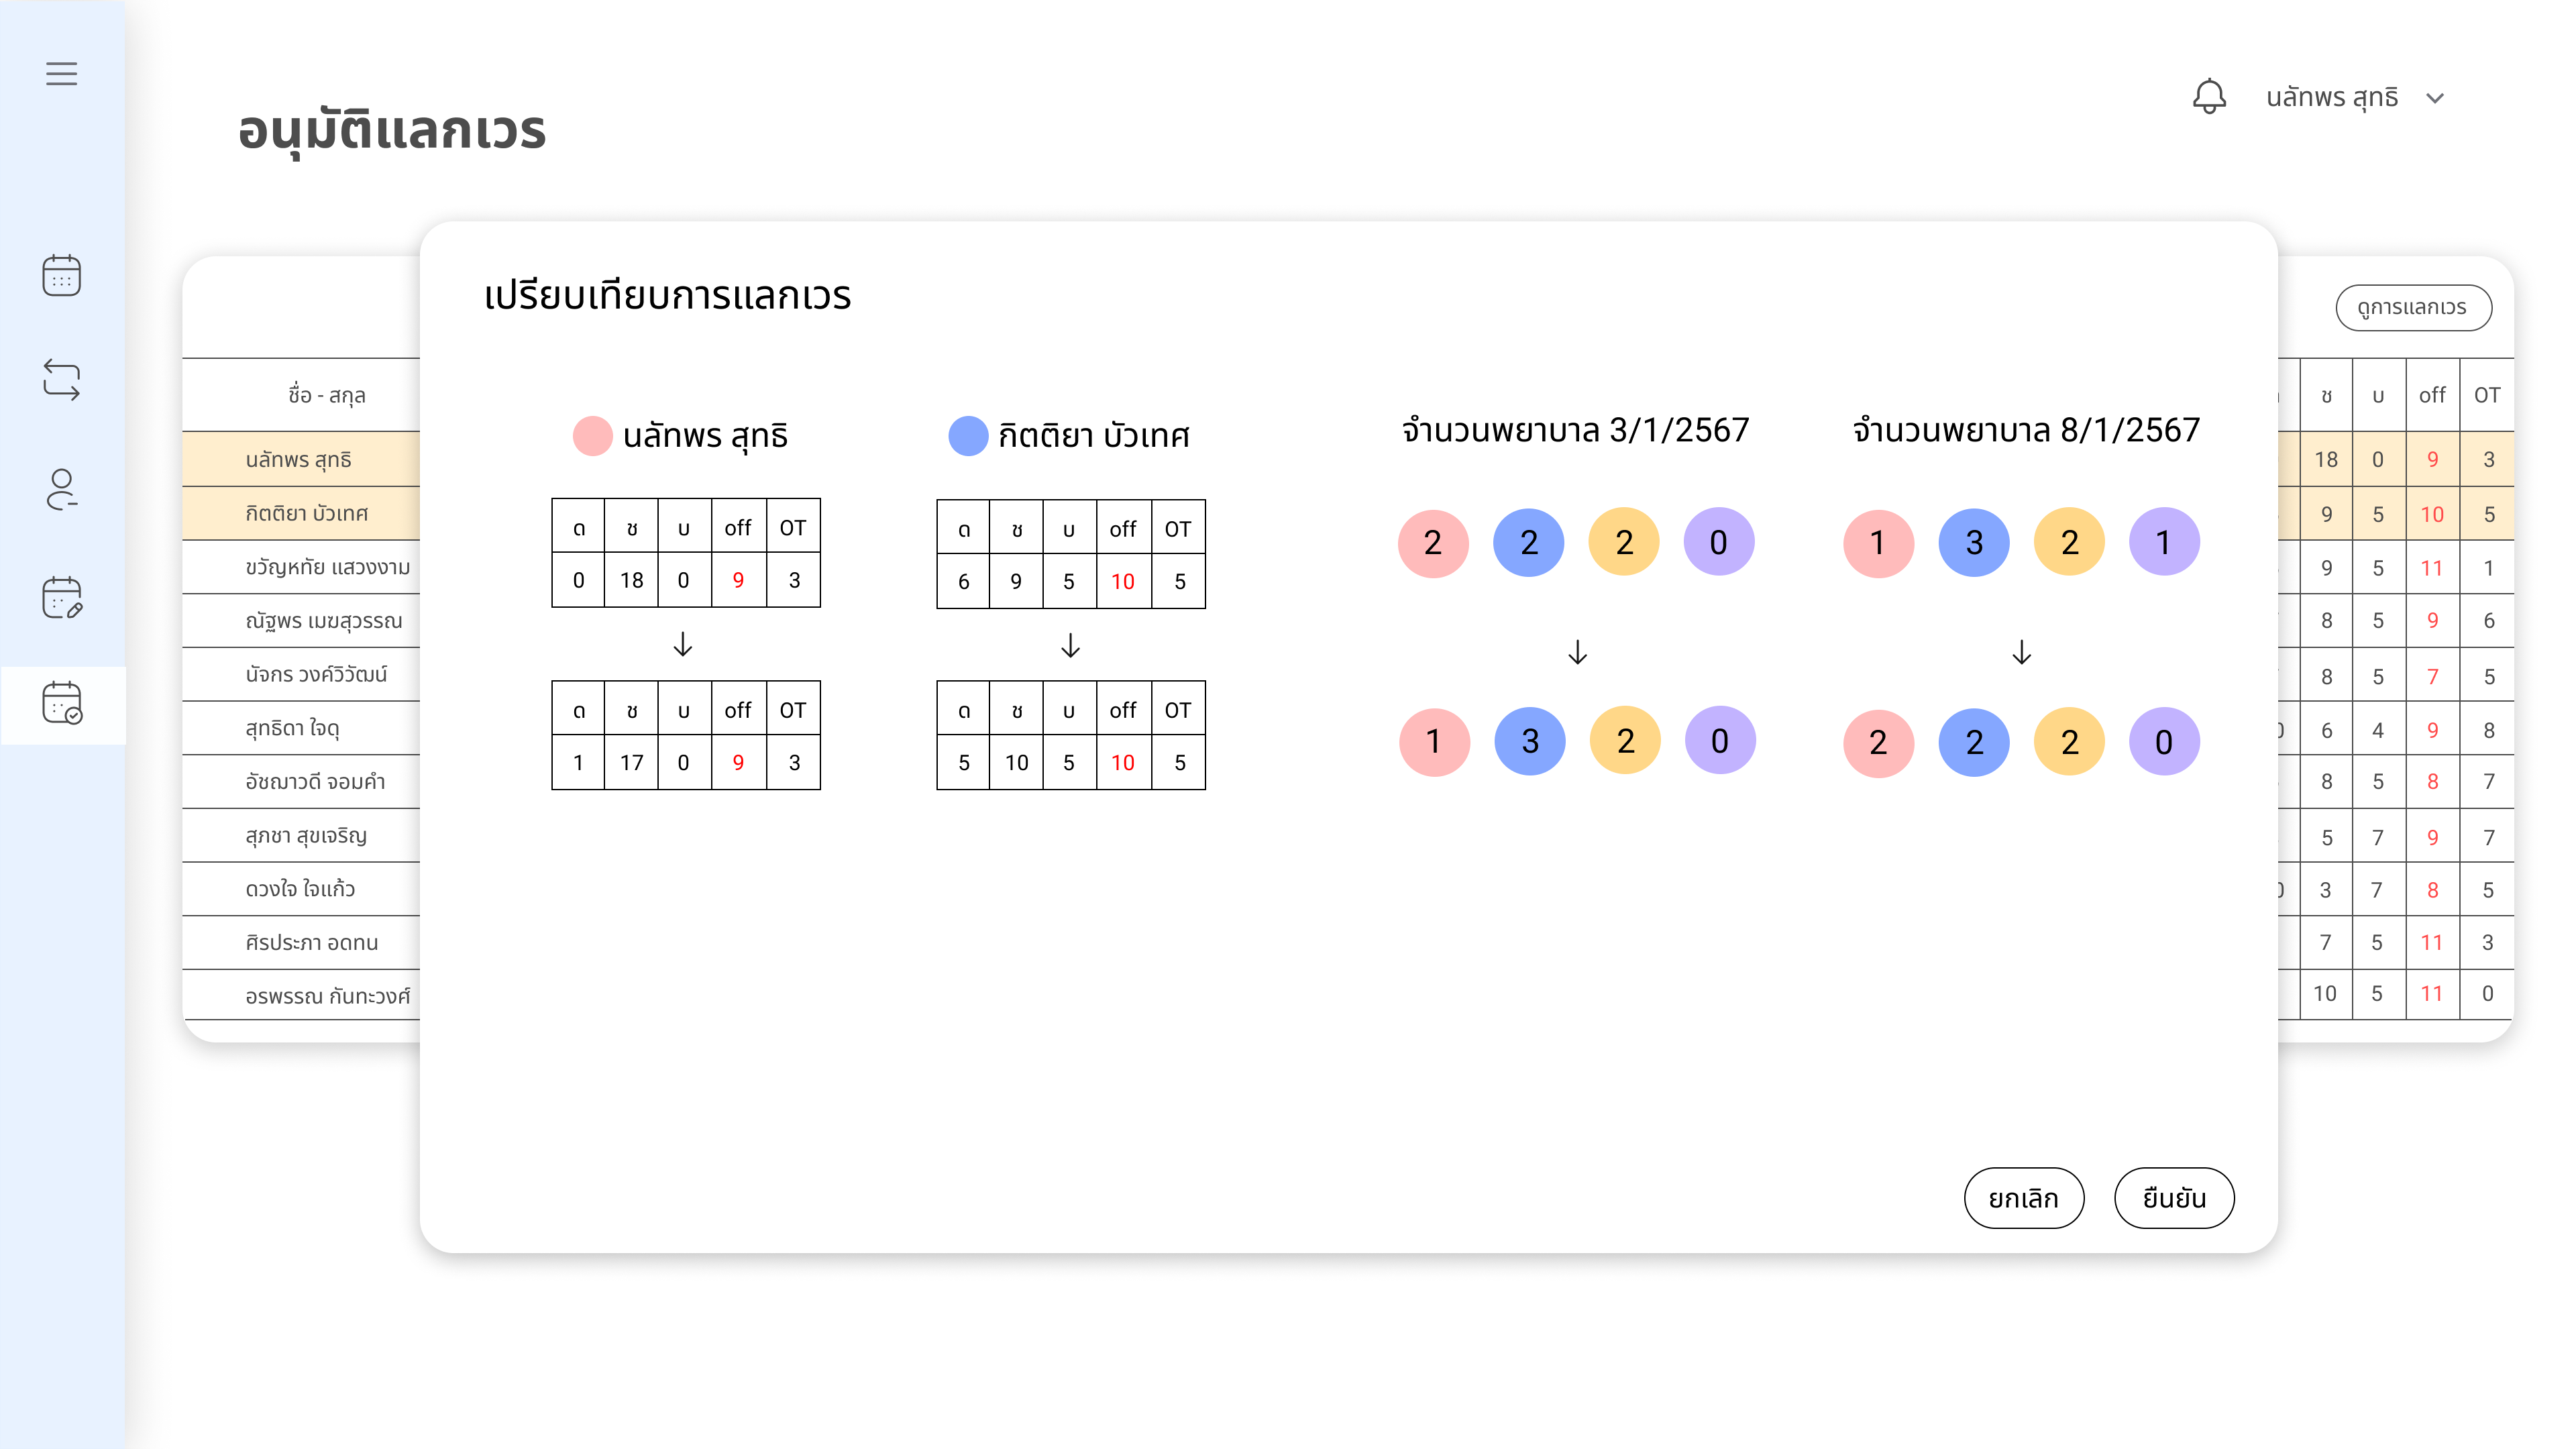
\includegraphics[width=0.8\textwidth]{9ui.png}
    \caption{แสดงหน้าเปรียบเทียบก่อนยืนยันการแลกเวร}
\end{figure}

\begin{figure}
    \centering
    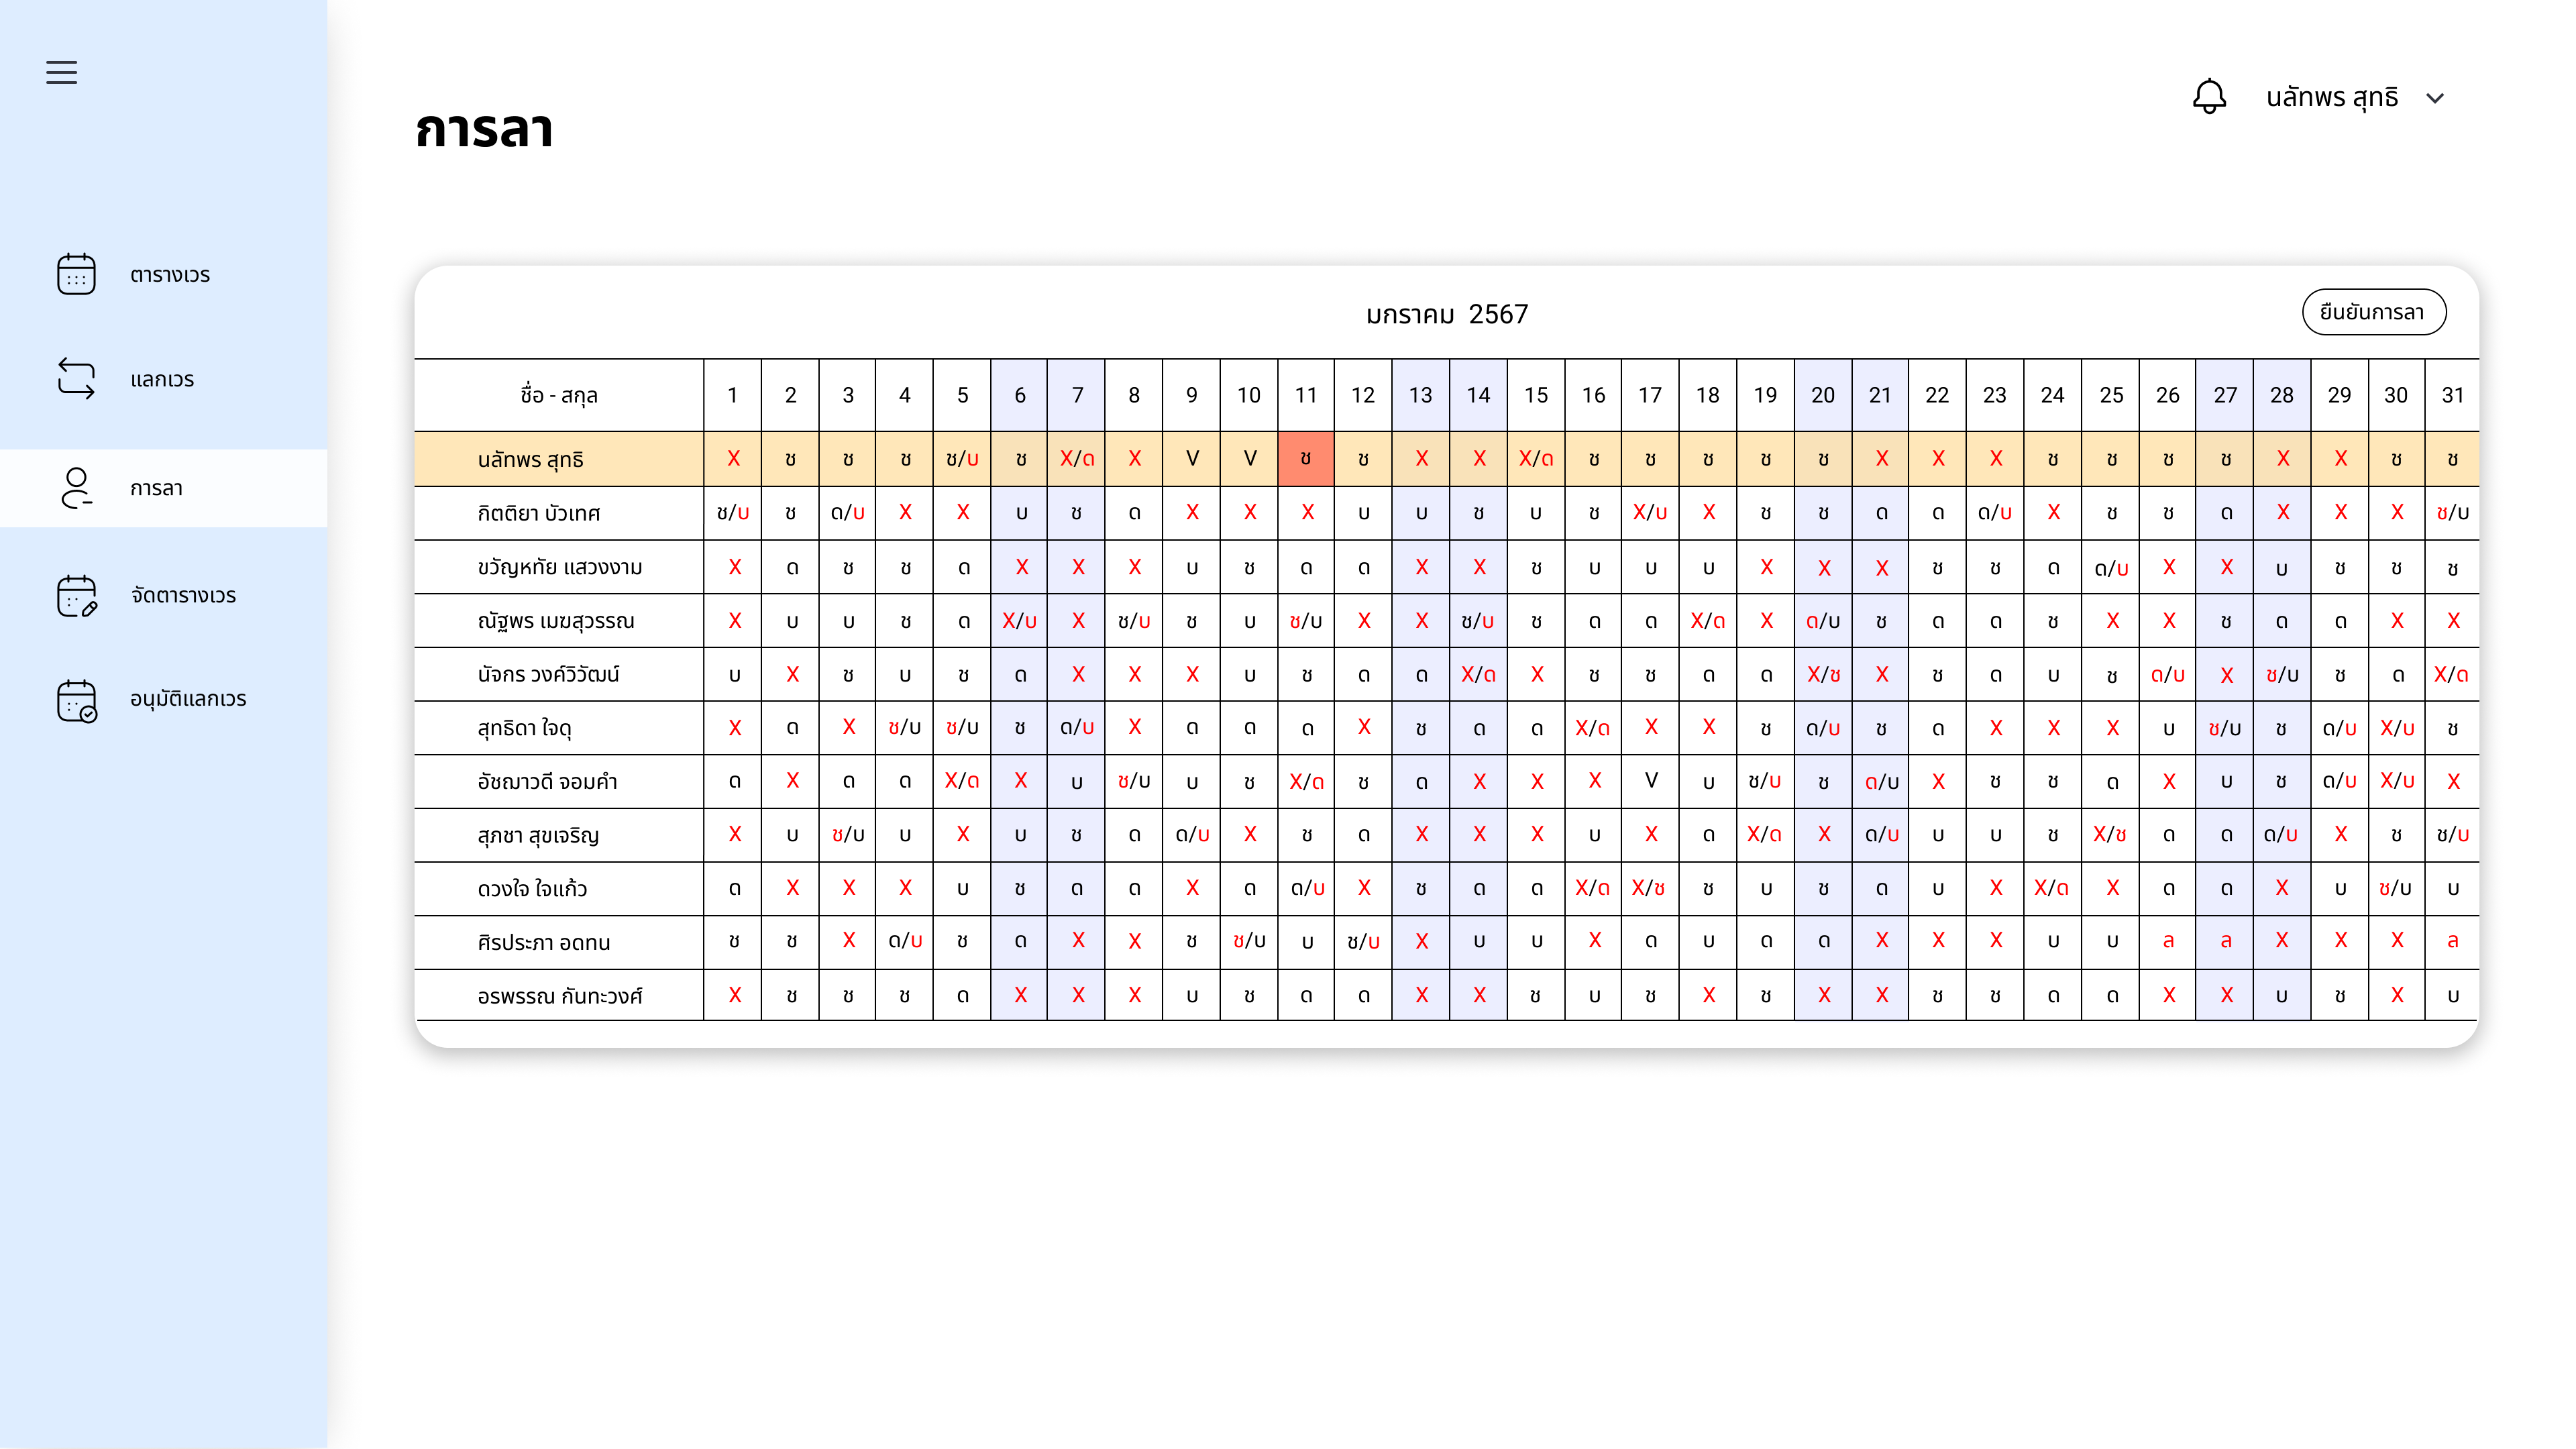
\includegraphics[width=0.8\textwidth]{10ui.png}
    \caption{แสดงหน้าการลา}
\end{figure}

\begin{figure}
    \centering
    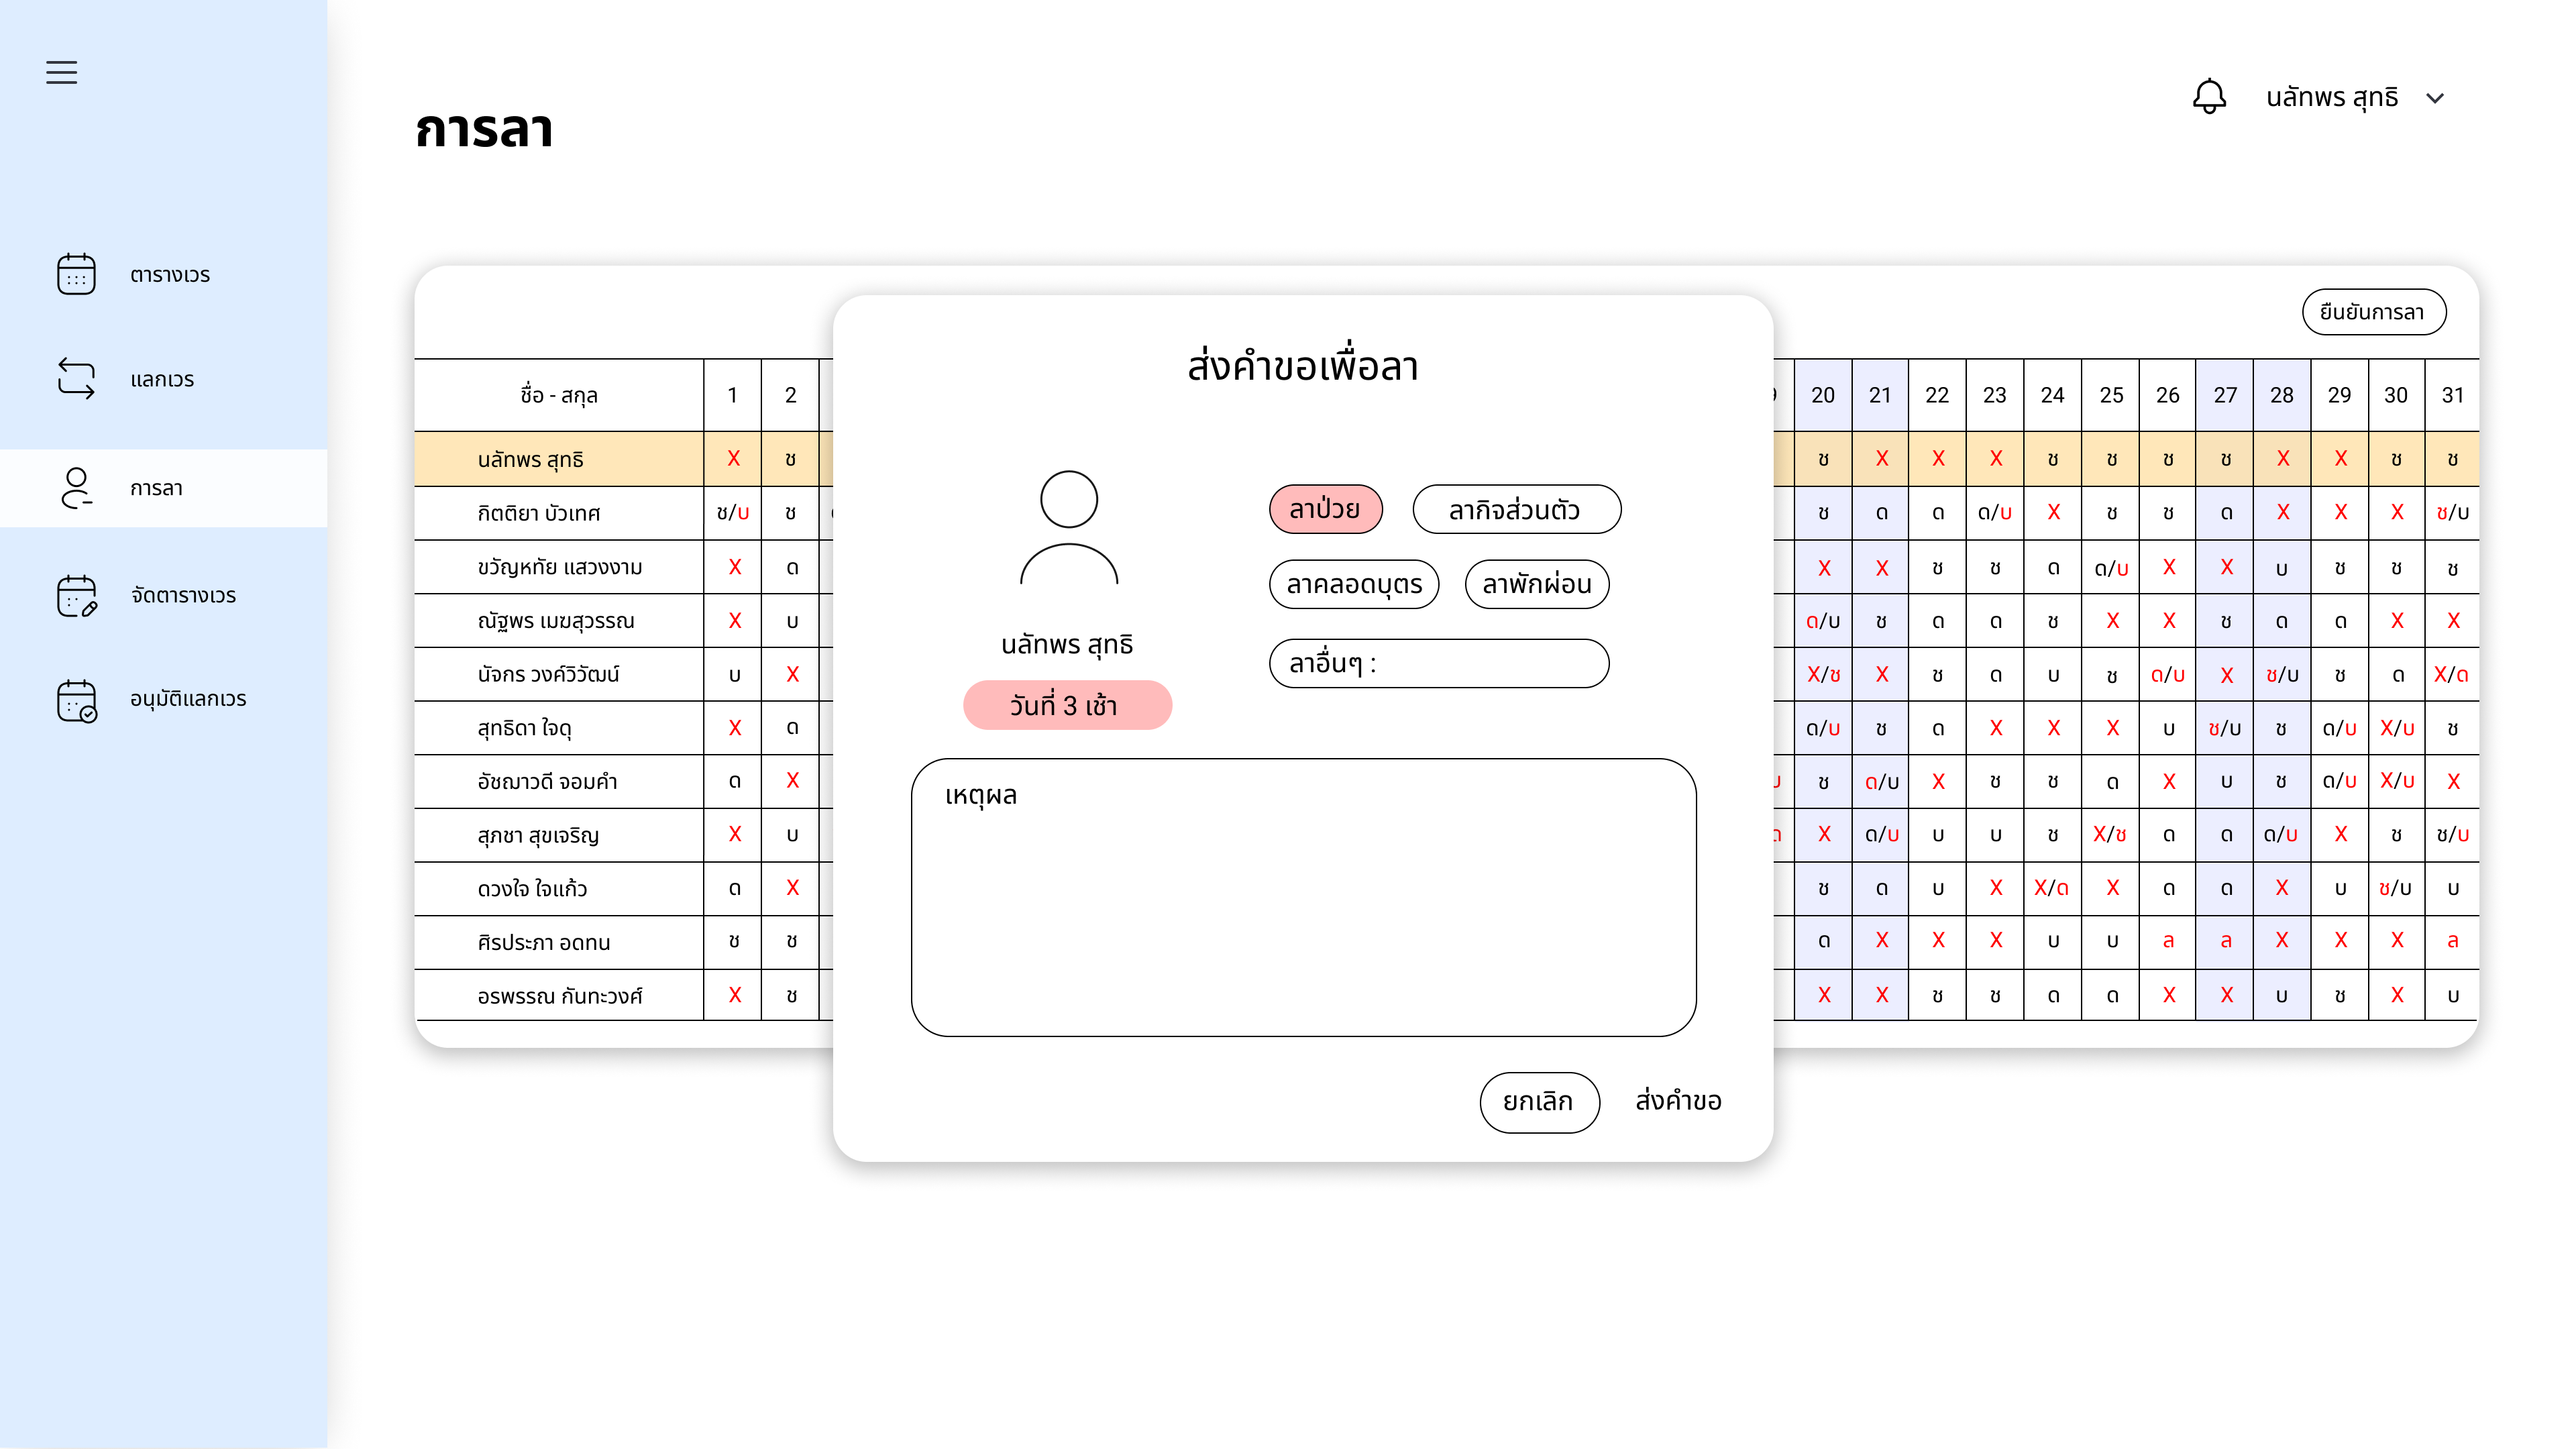
\includegraphics[width=0.8\textwidth]{ui11.png}
    \caption{แสดงหน้าการกรอกรายละเอียดลา}
\end{figure}
